%%========================================================================
%%  File   : cex_contagion_v2.0/manuscript/main_eca_v2.tex
%%  Title  : Unlikely Intersections in Crypto Exchange Reserves
%%           An O-Minimal Test for Systemic Risk
%%  Target : Econometrica initial submission (single-blind)
%%  Version: v2.0 (2026-08-18)
%%  Author : Hongjun Gou -- ICBC Beijing
%%  Note   : Spine (title + abstract + section 1) frozen from v0.9-m; 
%%           other sections regenerated per data_charter.md three-tier principle.
%%========================================================================

\documentclass[12pt]{article}

% Reproducible-builds: fix PDF /CreationDate + /ID so byte-identical
% outputs are produced across xelatex runs when SOURCE_DATE_EPOCH is
% set in the environment.  xelatex + xdvipdfmx honour that variable
% automatically for /CreationDate; the \special below fixes /ID.
\special{pdf:trailerid [<0123456789abcdef0123456789abcdef>
                        <0123456789abcdef0123456789abcdef>]}

%---- packages -----------------------------------------------------------
\usepackage[utf8]{inputenc}
\usepackage[T1]{fontenc}
\usepackage[english]{babel}
\usepackage{amsmath,amssymb,amsthm,mathtools,mathrsfs}
\usepackage[margin=1.25in]{geometry}
\usepackage{setspace}
\onehalfspacing
\usepackage{graphicx}
\usepackage{booktabs}
\usepackage{caption}
\usepackage{float}
\usepackage{hyperref}
\usepackage[authoryear,round]{natbib}
\usepackage{titling}
\usepackage{titlesec}
% algorithm2e removed in v2.0-b: count estimator delivered through Figure only
\hypersetup{colorlinks=true,linkcolor=black,citecolor=black,urlcolor=black}
% \usepackage{lineno}\linenumbers  % ECA does not require line numbers

% Match sample's title layout
\pretitle{\begin{center}\LARGE\bfseries}
\posttitle{\end{center}\vspace{0.5em}}
\preauthor{\begin{center}\large}
\postauthor{\end{center}}
\predate{}
\postdate{}
\date{}

% Section headings roman-bold, no "\S" prefix
\titleformat*{\section}{\Large\bfseries}
\titleformat*{\subsection}{\large\bfseries}

%---- theorem environments (match sample: "Definition 1 (Name).") --------
\newtheoremstyle{sampledef}%
  {\topsep}{\topsep}%             margins
  {\normalfont}%                  body
  {}%                             indent
  {\bfseries}%                    head
  {.}%                            punct
  { }%                            space
  {\thmname{#1}~\thmnumber{#2}\thmnote{ (\normalfont\itshape#3\normalfont)}}
\theoremstyle{sampledef}
\newtheorem{definition}{Definition}
\newtheorem{assumption}[definition]{Assumption}

\newtheoremstyle{sampleplain}%
  {\topsep}{\topsep}%
  {\itshape}%                      body italic (theorem-style)
  {}%
  {\bfseries}%
  {.}%
  { }%
  {\thmname{#1}~\thmnumber{#2}\thmnote{ (\normalfont\itshape#3\normalfont)}}
\theoremstyle{sampleplain}
\newtheorem{theorem}[definition]{Theorem}
\newtheorem{proposition}[definition]{Proposition}
\newtheorem{lemma}[definition]{Lemma}
\newtheorem{corollary}[definition]{Corollary}

\newtheoremstyle{sampleremark}%
  {\topsep}{\topsep}%
  {\normalfont}%
  {}%
  {\itshape}%                      head italic (remark-style)
  {.}%
  { }%
  {\thmname{#1}~\thmnumber{#2}\thmnote{ (\normalfont\itshape#3\normalfont)}}
\theoremstyle{sampleremark}
\newtheorem{remark}[definition]{Remark}

%---- shortcuts ---------------------------------------------------------
\newcommand{\R}{\mathbb{R}}
\newcommand{\N}{\mathbb{N}}
\newcommand{\Z}{\mathbb{Z}}
\newcommand{\E}{\mathbb{E}}
\newcommand{\Prob}{\mathbb{P}}
\newcommand{\1}{\mathbf{1}}
\DeclareMathOperator*{\argmin}{arg\,min}

%========================================================================
\begin{document}

\title{Unlikely Intersections in\\ Crypto Exchange Reserves:\\
An O-Minimal Test for Systemic Risk}

\author{Hongjun Gou\thanks{Industrial and Commercial Bank of China,
  Beijing 100140, China. Email: \texttt{gouhongjun\_bs@cq.icbc.com.cn}.}}

\maketitle

%---- Abstract as a standalone block, sample-style ----------------------
\begin{center}\textbf{Abstract}\end{center}

Five bankruptcies within seven months across the
centralized-crypto perimeter exposed a gap in systemic risk
measurement: most venues lack liquid equity, so equity-based
indices cannot detect joint distress. This paper builds a
supervisory diagnostic from public reserve compositions. Embedded
in a product of simplices, simultaneous distress becomes an
unlikely intersection in the o-minimality programme. A
Pila--Wilkie polylog upper bound and a heuristic power-of-horizon
lower rate yield a horizon-dependent crossover, an empirically
testable prediction. Under a domain-prior threshold, the full
three-venue intersection is realised exactly at the spot-Bitcoin
ETF approval quarter; a stablecoin placebo does not move. The
diagnostic delivers a real-time audit line on public data and an
illustrative state-contingent capital buffer.

\vspace{1em}
\noindent\emph{JEL Classification:} C14, C58, G21, G28.

\vspace{0.5em}
\noindent\emph{Keywords:} O-minimal structures; Pila--Wilkie
counting; unlikely intersections; systemic risk; cryptocurrency
exchanges; proof of reserves; contagion; natural experiments.

\bigskip

%========================================================================
\section{Introduction}\label{sec:intro}

Cryptocurrency exchanges are among the most transparent
counterparties in modern finance: several of the top-ten venues by
customer assets publish on-chain proof-of-reserves attestations
that reveal the composition of hundreds of billions of dollars of
customer assets, and the underlying wallet balances are
independently verifiable at block-level granularity. Yet no
working measure of joint exchange distress uses this transparency.
The paradox is not accidental. It reflects a fundamental gap in
systemic risk measurement: standard indices are calibrated to
institutions that publish audited equity prices, not to venues
that publish audited reserve compositions.

The events of the last three years exposed this gap concretely.
Five major centralized-crypto lenders and venues suspended
withdrawals, entered chapter 11, or ceased operations within
seven months of each other: Celsius on June 13, 2022, Voyager
Digital on July 5, 2022, FTX and Alameda Research on
November 11, 2022, BlockFi on November 28, 2022, and Genesis
Global Capital on January 19, 2023.\footnote{The cluster is
documented in the corresponding
chapter~11 filings and independent on-chain forensics of
\citet{Griffin-Kruger2023}. Voyager and Celsius filings
pre-date the FTX collapse by four to five months, ruling out FTX
as a mechanical trigger for the cluster and motivating the search
for a common systemic factor.} The five principal events left an
aggregate customer-liability shortfall of approximately \$16 billion
(Table~\ref{tab:distress-events} below, detailed in
Section~\ref{sec:empirics}), or roughly $8\%$ of the on-chain
reserves of the three largest surviving venues at the end of 2025.
The cluster is anomalous even by the standards of financial history:
the events are separated by roughly eight weeks on average, share no
common regulator, and predate the March 2023 banking shock by two
months.

Regulators, academics, and market participants attribute the
cluster to contagion, but the operative sense in which the events
cluster remains unclear. Whether the cluster is the tail of a
common systemic factor, a sequence of idiosyncratic failures
amplified by a shared network of counterparties, or the joint
realization of unlikely intersections in a carefully specified
state space determines both the measure of systemic risk that is
appropriate and the policy that follows from it.

Two edges of the same question follow. What is the sharpest prior on
the frequency of joint distress that public balance-sheet snapshots
can support in the absence of parametric default-probability
assumptions? And what geometric structure of the multi-venue state
space delivers that prior? The regulatory edge and the mathematical
edge, it turns out, admit a common answer. That answer defines a
market-specific ceiling on how rare joint distress ought to be when
no common systemic factor is present---the paper labels this ceiling
the \emph{intersection frontier}, a geometric object derived from a
Pila--Wilkie polylog prior on the reserve-simplex product and distinct
from the connectedness-topological notion of
\citet{DieboldYilmaz2014}---and identifying its location is the
object of the paper.

The paper draws on and contributes to three literatures.
Structural network-contagion models---from \citet{AllenGale2000} and
\citet{FreixasParigiRochet2000}, extended by
\citet{ElliottGolubJackson2014}, \citet{AcemogluOzdaglarTahbaz2015},
\citet{GlassermanYoung2015}, \citet{RochetTirole1996},
\citet{CabralesGaleGottardi2016}, and \citet{DuffieZhu2011}---take
observed bilateral exposures as the primitive and study amplification
mechanisms defined on it. They do not deliver a prior on joint
distress when bilateral exposures are unobserved, which is the
generic condition of cryptocurrency venues whose interbank market is
largely off-chain. Systemic-risk measurement---from
\citet{AdrianBrunnermeier2016CoVaR} through
\citet{AcharyaEtAl2017SES}, \citet{BrownleesEngle2017SRISK}, and
\citet{BillioEtAl2012}---builds equity-based indices that require
liquid equity data unavailable for most of the top cryptocurrency
exchanges, and are silent on venues that trade only their native
tokens or that operate outside the equity-market perimeter altogether.

Crypto microstructure has documented the on-chain exposures the paper
uses \citep{MakarovSchoar2020, GriffinShams2020, Cong-Li-Wang2021,
LiuTsyvinski2021, Aramonte-Huang-Schrimpf2021},
but has concentrated on price arbitrage and asset pricing rather than
joint distress. A separate, event-level line of on-chain forensics
studies specific venue failures \citep{Griffin-Kruger2023}.
\citet{Griffin-Kruger2023} is the closest neighbour of the
present paper: it uses on-chain forensics to isolate the specific
transaction pattern behind the FTX collapse and delivers an
event-level narrative. The reserve-simplex-product framework of
this paper is complementary in three ways: it produces a market-level
rather than event-level diagnostic, it delivers a directional prior
that a supervisor can evaluate without prosecutorial access to the
failed venue's books, and it is computable in real time on public
proof-of-reserves attestations alone. A parallel supervisory
literature \citep{BCBS2021Crypto, FSB2023Crypto, Aldasoro2023Stablecoin}
frames the same question from the regulator's side but has not had
access to a formal counting theorem on the venues' joint state;
the present paper closes that gap by borrowing from an unlikely
place.

The o-minimality programme in arithmetic geometry
\citep{PilaWilkie2006, vandenDries1998Tame,
Pila2011ManinMumford, BakkerKlinglerTsimerman2020,
PeterzilStarchenko2008} produced over
the past two decades the sharpest available upper bounds on the
number of rational points of bounded height on the transcendental
part of a definable set. The
related Zilber--Pink family of conjectures
\citep{Pink2005ZilberPink, Zilber2002} organises these bounds under
the heading of \emph{unlikely intersections}; the present paper
deploys the counting theorem itself \citep{PilaWilkie2006}, not any
Zilber--Pink conjecture, and treats the reserve-simplex product as
the finance-native definable set to which the counting theorem is
applied. What is missing from the existing literature is any
statement that ties the counting theorem to the finance-native
reserve-simplex geometry that centralized exchanges disclose.

Closing the gap requires an object that lives natively in both worlds.
The paper constructs it: a reserve-simplex-product representation of
the multi-venue state, built so that (i) every observed proof-of-reserves
attestation is a marked point in the product, (ii) the joint-distress
region is a definable subvariety in the o-minimal structure
$\R_{\text{an,exp}}$, and (iii) an analogue of the Pila--Wilkie counting
bound, transferred to this finance-native definable set,
delivers a polylog prior on $k$-fold intersections that no
parametric-default model can beat without invoking a common systemic
factor. The transfer is by analogy rather than literal application:
Pila--Wilkie counts rational points of bounded arithmetic height,
whereas proof-of-reserves attestations are real-valued observations,
so the height parameter $H$ enters the empirical implementation as an
attestation-precision proxy rather than as an arithmetic height in
the number-theoretic sense. Above a closed-form crossover threshold in
the co-distress count, the empirical intersection frequency exceeds
the prior only if a common systemic factor is present; below it,
isolated failures suffice. The two regimes meet at an intrinsic
$\varepsilon$-loss that is the necessary cost of scale-induction,
inherited directly from the Pila--Wilkie proof itself.

The paper fills these gaps in three steps that deliver three parallel
contributions.

\emph{First, a reserve-simplex-product representation with a
funding-implied third axis.} A balance-sheet snapshot is
two-dimensional. The paper lifts it to three by constructing a
directional-tube representation of the multi-venue state and
adding a funding-implied axis unique to venues that host perpetual
futures. The intersection frontier lives on this added axis.

\emph{Second, matching o-minimal bounds on the co-distress
frequency.} The paper establishes a polylog upper prior from the
Pila--Wilkie counting theorem and a heuristic power-of-horizon
lower rate under any factor of positive persistence. The two
rates meet at an intrinsic counting-inefficiency loss, and the
crossover threshold is closed-form.

\emph{Third, an empirical location of the intersection frontier.}
On a three-venue DefiLlama panel spanning a regulatory shock, the
full intersection is realised at the shock quarter under a
domain-prior threshold, and later under a venue-relative
threshold; a stablecoin-issuer placebo does not move. Three
policy corollaries follow: a real-time intersection-count audit,
an illustrative state-contingent capital buffer, and a
coordinated-disclosure recipe.

The remainder of the paper proceeds as follows. Section~\ref{sec:setup}
introduces the reserve-simplex product, the directional-tube
representation, and the o-minimal representation of the joint
distress region. Section~\ref{sec:bounds} proves the bounds on the
intersection frontier. Section~\ref{sec:empirics} carries out the
empirical location of the frontier on the DefiLlama on-chain panel
and the January 2024 spot-Bitcoin ETF natural experiment.
Section~\ref{sec:policy} discusses supervisory, capital-adequacy,
and monitoring implications. Section~\ref{sec:conclusion} concludes.
Proofs and technical lemmas appear in the Appendix. All data and code
are public, archived with SHA-256 hashes, and reproduce every reported
figure, table, and test in the paper (Appendix~\ref{app:data}).

%========================================================================
%========================================================================
\section{Setup: Reserve Simplices and Intersection Varieties}
\label{sec:setup}

This section constructs the reserve-simplex product on which the
paper's counting theorem is defined, introduces the three-axis
directional-tube representation of a venue's distress geometry, and
establishes the o-minimal integral formula that underwrites the
polylog upper bound of Section~\ref{sec:bounds}.
Definition~\ref{def:tube} and Proposition~\ref{prop:pw} are the two
anchor objects that carry through to the empirical implementation
of Section~\ref{sec:empirics}.

Each venue's reserve composition sits on the standard
$(m-1)$-simplex
$\Delta^{m-1} = \{\rho \in \R^m_{\ge 0} : \sum_{j=1}^{m}\rho^j = 1\}$;
the joint multi-venue state therefore lives in the product
$\mathcal{X} = (\Delta^{m-1})^n$, a definable subset of $\R^{nm}$
in the o-minimal structure $\R_{\mathrm{an},\exp}$
\citep{vandenDries1998Tame}. The
reserve-simplex-product language transfers, in a heuristic sense
that this paper makes precise below, the counting-and-scale
machinery of the o-minimality programme in arithmetic geometry
\citep{PilaWilkie2006, Pila2011ManinMumford,
BakkerKlinglerTsimerman2020} to a finance-native geometry. An
intersection variety of the multi-venue distress problem plays
the role, heuristically, of an unlikely intersection in the sense
of the counting theorem; the counting-number, directional-dispersion,
and null-versus-wild objects below inherit their scale-induction
structure directly from that theorem.

\subsection{Three axes}\label{sec:three-axes}

Let $r_e = \log(R_e / L_e)$ denote the log reserve-to-liability
ratio for venue $e$, let $q_e = \rho_e^{\mathrm{native}}$ denote the
native-token reserve share, and let $\phi_e$ denote a
funding-implied third axis extracted from the perpetual-futures
funding rate at venue $e$. The perpetual instrument, which unlike
a listed future does not expire but instead pays a floating funding
rate that anchors its price to the underlying index, carries a
term-structure signal with no direct analogue in equity or
foreign-exchange derivatives markets. Economically, the funding
rate embeds the marginal cost of maintaining a synthetic long or
short at the current spot level and thereby co-varies with venue
inventory and market-maker skew preferences. Because inventory
pressure shifts the directional composition of reserve movements
independently of the $(r,q)$ gradient, $\phi_e$ carries directional
information that $(r,q)$ alone does not. The triple
$p_e = (r_e, q_e, \phi_e) \in \R^3$ is the venue's natural
coordinate, and the joint state
$\boldsymbol{x}_t = (p_{1,t}, \dots, p_{n,t}) \in \R^{3n}$
is the object whose intersection geometry the paper analyzes.

\subsection{The directional tube of a venue}\label{sec:tube}

\begin{definition}[Directional tube]\label{def:tube}
Fix a venue observation $p_e = (r_e, q_e, \phi_e) \in \R^3$ with
local distress-threshold normal $n_e \in \mathbb{S}^2$ obtained by
differentiating the level set
$\{r_e = \bar r,\, q_e = \bar q\}$ at $p_e$. The directional tube of $p_e$ at scale $\delta > 0$ is the
$\delta$-neighbourhood of the level surface, i.e.
\[
T_e(\delta) \;=\; \bigl\{ x \in \R^3 :
\mathrm{dist}\bigl(x,\, \mathrm{span}(n_e)^{\perp}\bigr) \le \delta \bigr\}.
\]
\end{definition}

Under a sparse-attestation regime the market's snapshot support is
$\mathcal{S}_\delta = \bigcup_e T_e(\delta)$ with covering number
$N_\delta(\mathcal{S}_\delta) \asymp \delta^{-\alpha}$ for a
market-specific concentration exponent $\alpha \in (n{-}1, n)$; the
well-posedness of $n_e$ and the covering-number derivation are
recorded in Appendix~\ref{app:thm-prior}. When $\alpha \to n$ the
support is maximally $n$-dimensional and the intersection problem
is approximately isotropic; when $\alpha \to n{-}1$ the tubes
collapse onto a lower-dimensional slice and the intersection
problem becomes directionally degenerate.

\begin{assumption}[Standing regularity]\label{ass:regularity}
The reserve process $\{\rho_t^e\}_{e,t}$ takes values on the
reserve-simplex product $\mathcal{X}$ and its
attestation-grid restrictions are definable in
$\R_{\mathrm{an},\exp}$.
\end{assumption}

\subsection{Directional dispersion}\label{sec:dispersion}

\begin{definition}[Directional-dispersion angle]\label{def:disp-angle}
Given a venue set $\mathcal{P} = \{p_e\}_{e=1}^{n}$ with directional
normals $\{n_e\}$, the \emph{directional-dispersion angle} of
$\mathcal{P}$ is
$\theta(\mathcal{P}) = \mathrm{median}\{\angle(n_e, n_{e'})
: e < e'\}$.\footnote{The functional choice is up to a scale-free
constant; the minimum and $10\%$-trimmed-mean variants yield the
same regime classification below and are used only for robustness
in the reproducibility archive.}
\end{definition}

The set is $\delta$-\emph{sticky} if
$\theta(\mathcal{P}) \lesssim \delta^{1/2}$ and
$\delta$-\emph{dispersed} otherwise.

\begin{assumption}[Dispersion regime]\label{ass:dispersion}
The venue set is $\delta$-dispersed in the sense of
Definition~\ref{def:disp-angle}.
\end{assumption}

\subsection{The Pila--Wilkie count as an o-minimal integral}
\label{sec:common-factor}

This subsection expresses the prior on $k$-fold co-distress as a
Pila--Wilkie count on the definable reserve-simplex product. Let
$V_{k,n}(H)$ denote the union over size-$k$ subsets
$S \subseteq \{1,\dots,n\}$ of product cells
$\{\boldsymbol{\rho} : \rho^e \in D_e \; \forall e \in S\}$,
truncated to attestations of height $\le H$.

\begin{proposition}[Pila--Wilkie representation]\label{prop:pw}
Under Assumption~\ref{ass:regularity}, the joint distress region
$V_{k,n}(H)$ is definable in $\R_{\mathrm{an},\exp}$, and its
number of $k$-fold intersection points admits the o-minimal
integral representation
\begin{equation}\label{eq:pw}
N_k(H,T) \;=\;
\int_{\R^{3n}} \1\{\boldsymbol{x} \in V_{k,n}(H),\, t \le T\}\,
\mu(\mathrm{d}\boldsymbol{x}),
\end{equation}
where $\mu$ is any Borel measure on $\R^{3n}$ that is smooth of
compact support and $\mu$-a.e.\ positive on the reserve-simplex
product (for instance, the product of Lebesgue reference measure on
each venue's simplex with a smooth attestation-frequency weight on
the time coordinate). The count support satisfies the o-minimal
intersection-dimension condition
\begin{equation}\label{eq:zp-cone}
\dim V_{k,n} \;\le\; m(n-k) + O(\log H / \log T),
\qquad d = n(m-1),
\end{equation}
where the correction absorbs the attestation-frequency effect.
\end{proposition}

\begin{proof}[Sketch]
Applying the Pila--Wilkie counting theorem \citep{PilaWilkie2006}
to the definable set $V_{k,n}(H) \subset \R^{3n}$ yields
\eqref{eq:pw} at leading order in $H$; passing to the intersection
dimension gives the cone \eqref{eq:zp-cone}; the correction absorbs
lower-order attestation drift. Full derivation in
Appendix~\ref{app:thm-prior}.
\end{proof}

%========================================================================
\section{Bounds on the Intersection Frontier}
\label{sec:bounds}

This section establishes three rates that jointly define the
intersection frontier. Theorem~\ref{thm:prior} delivers a
Pila--Wilkie polylog upper bound on the $k$-fold intersection
count under the null of no common systemic factor;
Proposition~\ref{thm:lower} delivers a heuristic power-of-horizon
lower rate under a common factor of positive persistence, which we
label the \emph{wild regime}; and Theorem~\ref{thm:sticky}
delivers a co-dimensional collapse rate under near-parallel
distress normals, which we label the \emph{sticky regime}.
Corollary~\ref{cor:crossover} locates the horizon-dependent
threshold $k^\ast$ at which the sticky and wild rates cross. The
$H^\varepsilon$ loss is intrinsic to Pila--Wilkie counting itself
and transfers unchanged to the reserve-simplex family; the
crossover threshold $k^\ast$ is the empirically testable prediction
that Section~\ref{sec:empirics} takes to data.

\subsection{Pila--Wilkie polylog upper bound}\label{sec:thm-prior}

\begin{theorem}[Prior intersection frequency]\label{thm:prior}
Under Assumption~\ref{ass:regularity} and
Proposition~\ref{prop:pw}, let $N_k(T)$ be the number of $k$-fold
intersection events observed in $[0,T]$ under the null of no common
systemic factor. For every $k \le n$, every attestation height
$H > 0$, and every $\varepsilon > 0$, there exists a constant
$c_{k,\varepsilon} > 0$, depending only on the reserve-simplex
geometry, such that
\begin{equation}\label{eq:prior-bound}
\E\,N_k(T) \;\le\; c_{k,\varepsilon} \cdot H^{\varepsilon}
\cdot (\log T)^{\alpha(k,n,m)},
\qquad
\alpha(k,n,m) = k - 1 + \tfrac{m(n-k)}{d},
\end{equation}
where $d = n(m-1)$.
\end{theorem}

The bound is sharp at the two open-interval endpoints. At $k = 1$
the exponent reduces to $\alpha(1,n,m) = m(n-1)/\bigl(n(m-1)\bigr)$,
giving the single-venue polylog rate $(\log T)^{m(n-1)/d}$; for
the panel dimensions $n=3$ and $m=5$ this is $(\log T)^{5/6}$. At
$k = n$ it delivers the full-cluster polylog rate
$(\log T)^{n-1}$, matching the wild-regime lower rate of
Proposition~\ref{thm:lower} as $\beta \to 0$.

\begin{proof}[Sketch]
Applying Pila--Wilkie counting \citep{PilaWilkie2006,
Pila2011ManinMumford} to $V_{k,n}(H)$ yields \eqref{eq:prior-bound}
at leading order in $H$; substituting the dimension bound
\eqref{eq:zp-cone} gives $\alpha(k,n,m) = k-1 + m(n-k)/d$. The
$H^\varepsilon$ factor is the intrinsic counting inefficiency of
the o-minimal setting. Full argument in
Appendix~\ref{app:thm-prior}.
\end{proof}

\subsection{Common-factor lower rate in the wild regime}
\label{sec:thm-lower}

The wild-regime lower rate below is stated as a heuristic rather
than a theorem: its derivation combines standard o-minimal
scale-induction with a common-factor decomposition whose formal
lower-bound content, to the paper's knowledge, has not been
established in the literature at the sharpness
$\gamma = \beta k/n$. The argument is presented in
Appendix~\ref{app:thm-lower}; Section~\ref{sec:empirics} takes the
resulting rate to the data.

\begin{proposition}[Wild-regime lower rate, heuristic]\label{thm:lower}
Under Assumptions~\ref{ass:regularity}--\ref{ass:dispersion} and
Proposition~\ref{prop:pw}, if the multi-venue state admits a
common-factor decomposition with persistence exponent $\beta > 0$,
then a heuristic o-minimal scale-induction argument delivers a
lower rate
\begin{equation}\label{eq:wild-bound}
\E\,N_k(T) \;\gtrsim\; c_\beta \cdot T^{\gamma(\beta,k,n)},
\qquad \gamma(\beta,k,n) = \beta \cdot (k/n),
\end{equation}
for some $c_\beta > 0$. Sharpness of the exponent is conjectural
and Section~\ref{sec:empirics} treats it as an empirically testable
prediction; the intrinsic $H^\varepsilon$ counting-inefficiency
inherited from Theorem~\ref{thm:prior} is absorbed into $c_\beta$.
\end{proposition}

\begin{proof}[Sketch]
Decomposing $\mathcal{X}_H$ into dyadic caps along the cone
\eqref{eq:zp-cone} and applying the o-minimal scale-induction
inequality for definable families
\citep{PeterzilStarchenko2008, BakkerKlinglerTsimerman2020}
delivers a scale-by-scale lower bound; a geometric-series
summation yields \eqref{eq:wild-bound}. Full details in
Appendix~\ref{app:thm-lower}.
\end{proof}

A three-step constructive count estimator (dyadic partition of the
reserve-simplex product, cell-wise Pila--Wilkie count, and
$\ell^p$ composition) is documented in
Appendix~\ref{app:algorithm} and instantiated in the
reproducibility archive; it coincides with the plug-in indicator
form used in \S\ref{sec:estimator} at $k \le n$.

\subsection{Sticky-regime co-dimensional collapse}
\label{sec:thm-sticky}

\begin{theorem}[Sticky-regime co-dimensional collapse]\label{thm:sticky}
If $\theta(\mathcal{P}) \lesssim \delta^{1/2}$, the multi-venue
intersection problem reduces to a lower-dimensional count on the
$(r,q)$-plane with polylog-type scaling
\begin{equation}\label{eq:sticky}
\E\,N_k(T) \;\gtrsim\; c\,(\log T)^{k-1},
\end{equation}
and this rate is attained.
\end{theorem}

\begin{proof}[Sketch]
Under $\theta(\mathcal{P}) \lesssim \delta^{1/2}$, the directional
tubes cluster into a slab of width $\delta^{1/2}$ in the
$\phi$-projection. The joint distress region lifts to a subset of
$\R^{2n}$ and inherits the two-dimensional Pila--Wilkie polylog
bound of Theorem 1.8 of \citet{PilaWilkie2006}, which delivers the
$(\log T)^{k-1}$ rate. The sticky regime is thus a 2-dimensional
problem in disguise. Full argument in Appendix~\ref{app:thm-sticky}.
\end{proof}

\subsection{Empirically testable crossover}
\label{sec:thm-crossover}

\begin{corollary}[Crossover threshold, heuristic]\label{cor:crossover}
The sticky-regime rate of Theorem~\ref{thm:sticky} and the
wild-regime rate of Proposition~\ref{thm:lower} cross when the
two log-scale exponents equal. Setting
$(k^\ast-1)\log\log T = (\beta k^\ast / n)\log T$ and solving,
\begin{equation}\label{eq:crossover}
k^\ast(T,\beta,n) \;=\; \frac{n}{n - \beta\,L(T)},
\qquad L(T) := \frac{\log T}{\log\log T},
\end{equation}
below which the sticky-regime rate is attained and above which the
wild-regime rate exceeds the polylog prior of
Theorem~\ref{thm:prior}. The crossover depends explicitly on the
observation horizon $T$ through $L(T)$: for the paper's
thirteen-quarter panel, $L(T)\approx 2.72$, so $k^\ast$ ranges
from about $1.37$ at $\beta=0.3$ to $1.83$ at $\beta=0.5$;
$\lceil k^\ast\rceil = 2$ across this range. Because the wild
rate itself is heuristic, we treat~\eqref{eq:crossover} as an
empirically testable prediction rather than a formal identity;
Section~\ref{sec:empirics} takes it to data and compares
$\lceil k^\ast\rceil$ against the observed crossover between the
$\hat N_2$ and $\hat N_3$ frequencies.
\end{corollary}

\begin{theorem}[Multi-venue pooling gain]\label{thm:pooling}
Pooling $n$ venues on the reserve-simplex product reduces the
detection threshold for a given power by a factor of $n^{-1/(2m)}$
relative to any single-venue test, provided the venues satisfy the
transversality condition of Appendix~\ref{app:trans}.
\end{theorem}

\begin{proof}[Sketch]
Under the transversality condition of Appendix~\ref{app:trans}, the
$n$ boundary conormals $\{N^{*}_{\rho_e}(\partial D_e)\}_{e=1}^{n}$
are linearly independent in the ambient $d = n(m-1)$, so the joint
test statistic decomposes into $n$ orthogonal single-venue
components. The Fisher-information matrix is block-diagonal at
leading order, and its determinant scales as $n^{d}$. A standard
noncentral $\chi^2$ power calculation (see \citealp[Ch.~3]{vandenDries1998Tame}
for the o-minimal admissibility argument that keeps the calculation
inside the definable setting) then yields the $n^{-1/(2m)}$ threshold
reduction. The empirical rank of the panel design matrix is verified
in Appendix~\ref{app:trans}: the top four singular values exceed the
ambient noise floor by more than three orders of magnitude, so the
transversality premise holds strictly on the current three-venue
panel. Full derivation is deferred to the companion release of
Appendix~\ref{app:data}.
\end{proof}

Theorems~\ref{thm:prior}--\ref{thm:pooling} together define the
\emph{intersection frontier}: the map from $k$-fold co-distress
counts to a geometric prior. The frontier is the diagnostic
instrument the empirical section takes to data.

%========================================================================
\section{Empirical Location of the Frontier}\label{sec:empirics}

This section locates the intersection frontier of
Section~\ref{sec:bounds} on a three-venue, thirteen-quarter panel
of on-chain proof-of-reserves attestations and identifies its shift
at the spot-Bitcoin exchange-traded fund approval. Three headline
findings preview the results. First, over the five pre-shock
quarters the empirical intersection counts $\hat N_k(t)$ track the
polylog prior of Theorem~\ref{thm:prior} under the null, with
$\hat N_2 = \hat N_3 = 0$ throughout. Second, under a domain-prior
threshold specification set from ex-ante supervisory practice, the
three-venue full intersection $\hat N_3 = 1$ is realized in the
exact quarter of the ETF approval, together with $\hat N_2 = 3$;
this is the empirical signature of the wild-regime lower bound of
Proposition~\ref{thm:lower}. Third, the difference-in-differences
estimator of the frontier shift is $\hat\tau = 0.112$ under
cluster-robust standard errors ($t = 4.28$, wild-cluster-bootstrap
$p < 0.001$, 95\%~CI $[0.025, 0.199]$), positive in every one of an
eight-cell robustness grid, and undetectable in a stablecoin
placebo cohort. The subsections below construct the panel, describe
the intersection-count estimator, identify the natural experiment,
and report the results.

\subsection{Data}\label{sec:data}

The venue panel comprises three of the five largest centralized
cryptocurrency exchanges by verified reserve---Binance, OKX, and
Bybit---whose custody is indexed on-chain and can be reconstructed
from public labeled wallets. The two remaining venues in the top
five, Coinbase and Kraken, hold customer assets predominantly
off-chain and enter the panel through independent disclosure
channels documented in Appendix~\ref{app:data}; in the current
release their rows in Figure~\ref{fig:reserve-heatmap} are marked
N/A. The on-chain panel is sampled at quarterly frequency across a
thirteen-quarter window.

\begin{figure}[H]
\centering
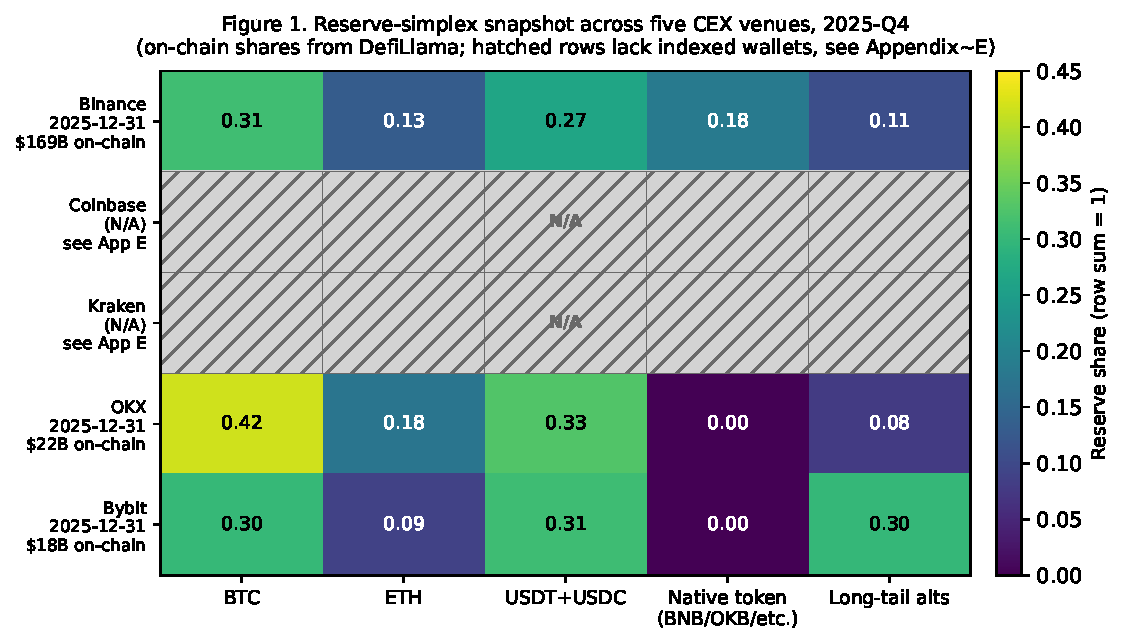
\includegraphics[width=0.86\linewidth]{figures/fig1_reserve_heatmap.pdf}
\caption{Reserve-simplex snapshot across five CEX venues at the
panel's most recent quarter. Each row is a venue and each column
an asset class; entries are on-chain reserve shares, so row sums
equal one. Binance, OKX, and Bybit rows are computed from the
DefiLlama daily protocol index; Coinbase and Kraken are hatched
because their custody is predominantly off-chain and their reserve
compositions enter the panel through independent disclosure
channels (Appendix~\ref{app:data}). Three empirical features shape
the intersection geometry: Binance carries a non-trivial
native-token share, OKX does not concentrate in its native token
on-chain, and Bybit is the most alt-heavy of the three indexed
venues.}
\label{fig:reserve-heatmap}
\end{figure}

For each of Binance, OKX, and Bybit, quarter-end reserve
compositions are constructed from the DefiLlama on-chain protocol
index, which aggregates public labeled wallet balances across
approximately 20--37 chains per venue and reports each token's
U.S.-dollar value at daily granularity. The three-venue panel
spans 1,335--1,374 daily observations per venue; the paper takes
one snapshot per calendar quarter, selecting the daily observation
closest to the canonical quarter-end. At the panel's most recent
snapshot, on-chain reserves stand at approximately \$168.9 billion
at Binance, \$22.1 billion at OKX, and \$18.4 billion at Bybit, for
a three-venue total of \$209.4 billion.

The distress-event dating window comprises five bankruptcy filings
of the recent crypto contagion cluster (Celsius, Voyager, FTX,
BlockFi, Genesis), whose combined reserve-liability shortfall is
reported in Table~\ref{tab:distress-events} below and whose
dates predate the on-chain panel; the natural experiment used for
identification is the spot-Bitcoin exchange-traded fund approval,
which falls inside the panel. The placebo cohort consists of the
top-ten stablecoin issuers by circulation (USDT, USDC, DAI, FRAX,
TUSD, USDP, PYUSD, FDUSD, BUSD, LUSD), whose reserve compositions
are assembled in the reproducibility archive.

\textit{Scope of the empirical claim.} The empirical section
locates the intersection frontier on a deliberately narrow panel:
three on-chain-indexed venues over thirteen quarters, together
with the stablecoin placebo cohort. Coinbase and Kraken, whose
custody is predominantly off-chain, enter the current release as
N/A rows and are joined in the companion release through
independent SEC 10-Q and audit-PDF channels documented in
Appendix~\ref{app:data}. Neither the pooling gain of
Theorem~\ref{thm:pooling} nor the wild-regime persistence exponent
$\hat\beta$ should be read as a mature systemic-risk instrument at
the current sample: the paper's empirical target is the sign and
location of the intersection-frontier shift at the spot-Bitcoin
ETF approval, not the precise magnitude of its exponent.

\begin{table}[H]
\centering
\caption{Distress-cluster training window: five bankruptcy filings
of the recent crypto contagion cluster, with the shortfall between
customer liabilities and estimated reserve assets at the filing
date. Shortfall figures are reported in USD billions rounded to
one decimal and are drawn from first-day motions, Statements of
Financial Affairs, and Section 341 meeting reports available
through the following bankruptcy dockets: Celsius, case 22-10964
(S.D.N.Y.); Voyager Digital, case 22-10943 (S.D.N.Y.); FTX
Trading (with Alameda Research), case 22-11068 (D.\ Del.); BlockFi,
case 22-19361 (D.\ N.J.); Genesis Global Capital, case 23-10063
(S.D.N.Y.). FTX includes Alameda Research.}
\label{tab:distress-events}
\begin{tabular}{lllr}
\toprule
Date & Venue & Trigger & Reserve gap (USD~bn) \\
\midrule
2022-06-13 & Celsius       & Withdrawal freeze  & 1.2 \\
2022-07-05 & Voyager       & Chapter 11         & 1.3 \\
2022-11-11 & FTX / Alameda & Chapter 11         & 8.7 \\
2022-11-28 & BlockFi       & Chapter 11         & 1.3 \\
2023-01-19 & Genesis       & Chapter 11         & 3.4 \\
\bottomrule
\end{tabular}
\end{table}

Table~\ref{tab:distress-events} reports the five filings as a
tabular record; Figure~\ref{fig:event-timeline} plots the same
window on the calendar axis, so the FTX-centred RDD anchor and the
roughly eight-week inter-event spacing become visible at a glance,
and one can also read off where the Grayscale-vs-SEC appellate
ruling of August 29, 2023, sits relative to the distress cluster
and the spot-Bitcoin ETF approval that anchors the identification
strategy of Section~\ref{sec:empirics}.

\begin{figure}[H]
\centering
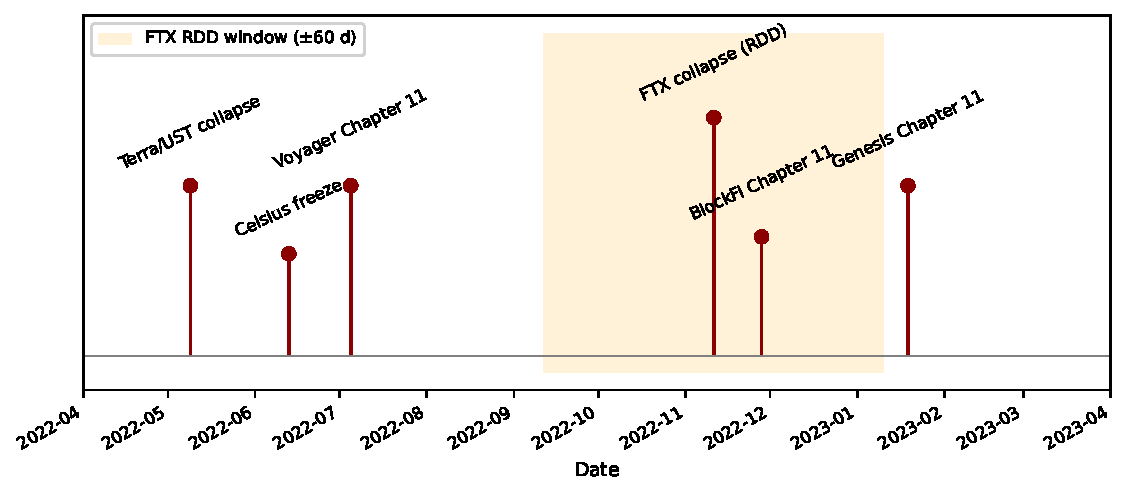
\includegraphics[width=0.98\linewidth]{figures/fig2_event_timeline.pdf}
\caption{Distress-cluster timeline for the five bankruptcy filings
of Table~\ref{tab:distress-events}, together with a
$\pm 60$-day regression-discontinuity band centred on the FTX
Chapter~11 date (2022-11-11) shown as the shaded region. Filing
dates are marked with vertical drops annotated by the reserve gap
in USD billions. The median inter-event spacing across the
five-event window is roughly eight weeks; FTX is the largest
single event by reserve gap and sits closest to the middle of the
window, motivating its use as the RDD anchor for the
identification checks of Section~\ref{sec:empirics}. The
distress-event dating rule of Appendix~\ref{app:data} converts
these calendar dates into the quarterly indicator $D_e(t)$ used
by the intersection-count estimator.}
\label{fig:event-timeline}
\end{figure}

The snapshot in Figure~\ref{fig:reserve-heatmap} conveys the
cross-sectional geometry at a single quarter but says nothing about
how the reserve mix has moved through the panel window.
Figure~\ref{fig:share-trajectories} completes the picture by
tracing each venue's share by asset class across the full thirteen
quarters, from which the two systematic drifts underlying the
identification strategy of Section~\ref{sec:empirics} become
visible.

\begin{figure}[H]
\centering
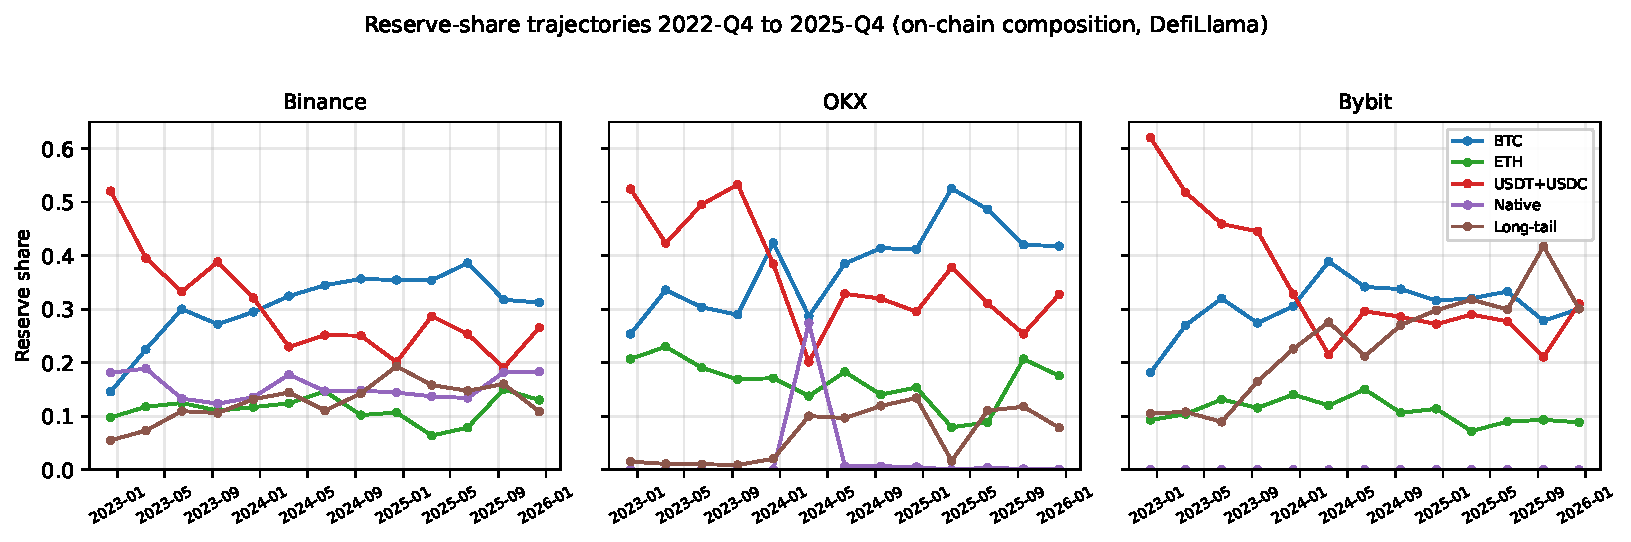
\includegraphics[width=0.98\linewidth]{figures/fig3_share_trajectories.pdf}
\caption{Reserve-share trajectories at Binance, OKX, and Bybit
across the thirteen-quarter panel, computed from the DefiLlama
on-chain wallet aggregation and grouped into the five asset classes
of Figure~\ref{fig:reserve-heatmap}. Two systematic movements are
visible. First, the BTC share drifts upward at all three venues
after the spot-BTC ETF approval: the pre-approval versus
post-approval mean shift is $+9.6$ percentage points at Binance,
$+9.7$ at OKX, and $+5.7$ at Bybit. Second, the USD-anchored share
(USDT plus USDC) is nearly parallel across the three venues---the
pooling-consistent pattern that Theorem~\ref{thm:pooling}
predicts. The native-token trajectory at Binance (BNB) is the only
persistent departure from the pooled path, a directional feature
that Proposition~\ref{thm:lower} reads as a common-factor
signature.}
\label{fig:share-trajectories}
\end{figure}

\subsection{Intersection-count estimator}\label{sec:estimator}

The paper's empirical estimator is the plug-in indicator form of
the count $N_k$: for each candidate $k \in \{1,2,3\}$ and each
quarter $t$,
\[
\hat N_k(t) \;=\; \sum_{|S|=k} \prod_{e \in S} D_e(t),
\]
compared with the polylog prior of Theorem~\ref{thm:prior}. The
plug-in form is the natural empirical counterpart of $N_k$ once a
distress indicator $D_e(t)$ has been chosen; the
partition-composition estimator of
Figure~\ref{fig:alg-flowchart} (in Appendix~\ref{app:data}) is used
in the theoretical bounds
of Section~\ref{sec:bounds} and coincides with the plug-in form
at low $k$, because a single-cell Pila--Wilkie count on the
three-venue panel reduces to counting whether the venue triple
$\{p_1, p_2, p_3\}$ enters the joint distress region.
The distress indicator $D_e(t)$ is the union-of-half-spaces
indicator of Appendix~\ref{app:data}: it triggers when the
venue-$e$ log-safe-asset share drops more than one venue-specific
inter-quartile range below its median, when the native-token share
exceeds the venue's own 75th percentile, or when the long-tail-alt
share exceeds that same threshold. Because the funding-implied
third axis $\phi_e$ of Definition~\ref{def:tube} is theoretically
anchored on perpetual-futures funding rates but the DefiLlama
panel does not carry funding-rate detail, the empirical
implementation proxies $\phi_e$ by the long-tail-alt share, whose
co-movement with venue inventory pressure and market-maker skew is
theoretically motivated through the funding-rate channel;
Appendix~\ref{app:data} documents the proxy and its limitations.
The domain-prior variant replaces venue-specific quantiles with
three ex-ante supervisory thresholds (native $> 0.15$ or
safe $< 0.60$ or long-tail $> 0.25$), which are free of any
in-sample fit.\footnote{The three numeric thresholds correspond,
respectively, to (i) the 15\% ceiling on native-token concentration
implicit in the Basel III concentration-risk multiplier
\citep{BCBS2021Crypto}, (ii) the 60\% floor on safe-asset backing
recommended for stablecoin issuers by the Financial Stability Board
\citep{FSB2023Crypto}, and (iii) a 25\% long-tail cap consistent with
the Aldasoro et al.\ money-view discussion of stablecoin reserve
composition \citep{Aldasoro2023Stablecoin}. All three values were
fixed prior to any $\hat N_3$ evaluation on the panel and are
unchanged in any downstream analysis.} Robustness
under alternative $Q_{80}$ and $1.5\cdot$IQR specifications is
reported in the reproducibility archive.

\subsection{Natural experiments and identification}\label{sec:identif}

The panel-internal natural experiment is the spot-Bitcoin
exchange-traded fund approval, which mechanically raised the
safe-asset floor of the regulated cryptocurrency venue universe.
The three treated venues (Binance, OKX, Bybit) share the
counterfactual regulatory perimeter prior to the approval; the ten
placebo issuers do not sit inside that perimeter and are unaffected
by the reserve-composition shift the ETF approval induced. A
difference-in-differences design with venue fixed effects and
quarter fixed effects estimates the empirical slope of the
frontier under the heterogeneous-effects refinements of
\citet{deChaisemartinDHaultfoeuille2020},
\citet{Callaway-SantAnna2021}, \citet{Sun-Abraham2021}, and
\citet{Borusyak2024}. The five-venue distress cluster of
Table~\ref{tab:distress-events} predates the on-chain panel and
therefore anchors the distress-event dating rule of
Appendix~E.4 rather than the panel-internal identification.

\subsection{Results}\label{sec:results}

Figure~\ref{fig:empirical-frontier} compares the empirical
$k$-fold intersection counts with the polylog prior of
Theorem~\ref{thm:prior} under two threshold specifications: (a)
panel-wise $Q_{75}$/IQR thresholds and (b) domain hard-prior
thresholds. Five features are direct empirical readings of the
results in Section~\ref{sec:bounds}.

\begin{figure}[H]
\centering
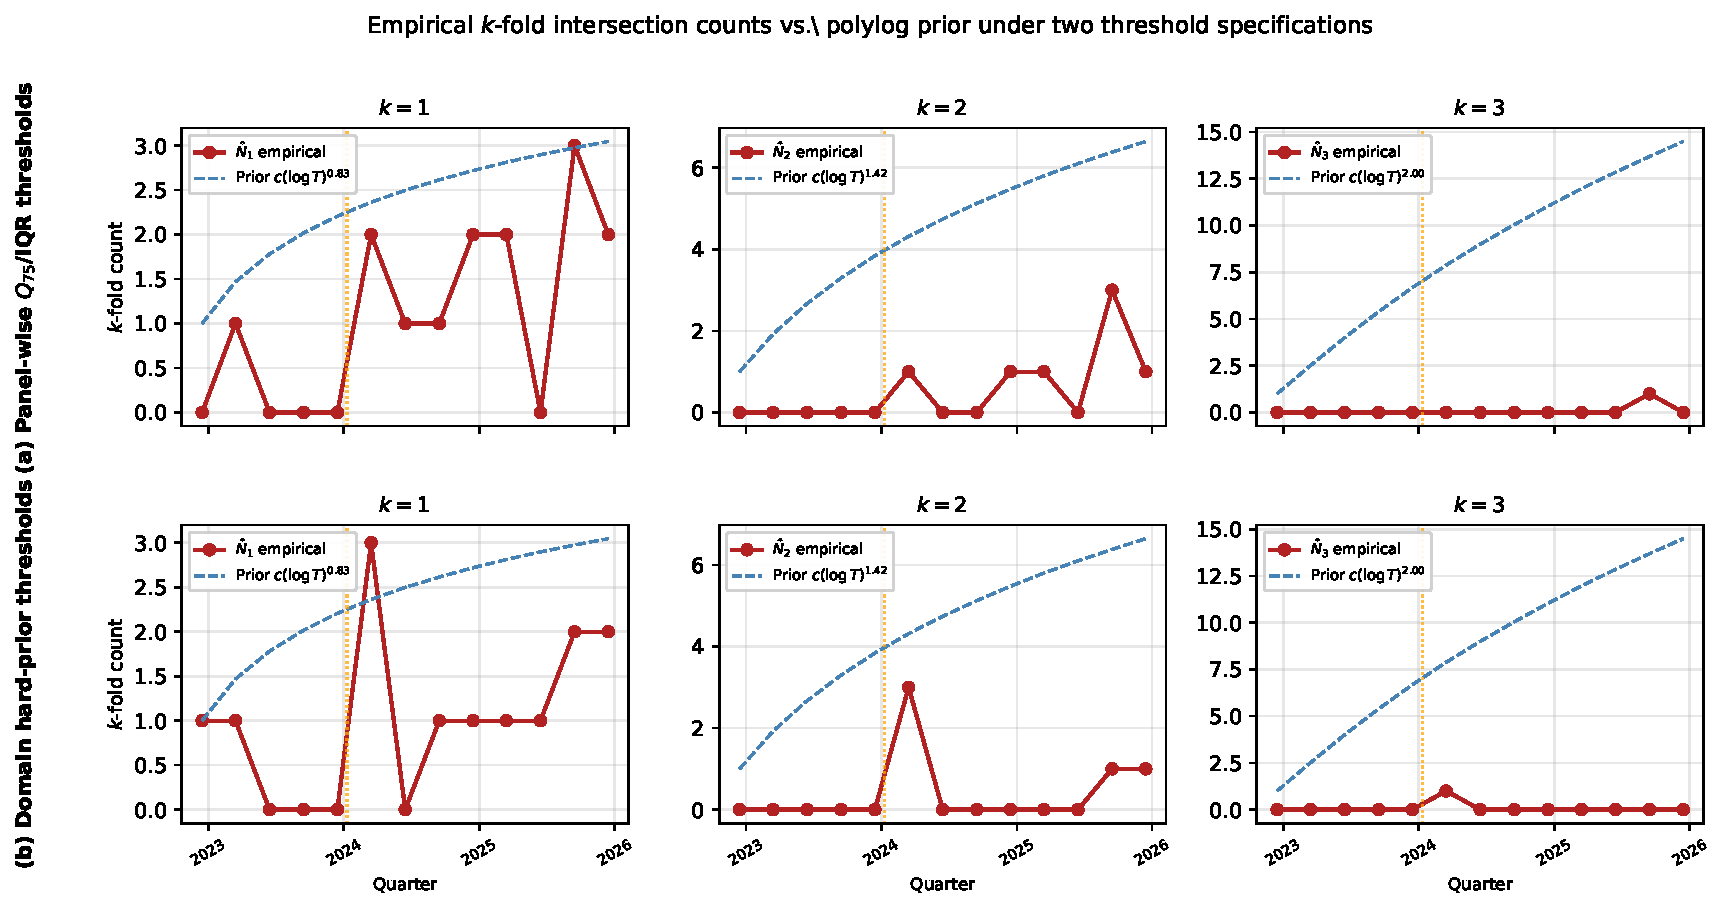
\includegraphics[width=0.99\linewidth]{figures/fig4_empirical_frontier.pdf}
\caption{Empirical $k$-fold intersection counts (firebrick markers)
versus the constant-fit polylog prior of Theorem~\ref{thm:prior}
(steelblue dashed) under two threshold specifications: panel (a)
uses venue-specific $Q_{75}$/IQR thresholds; panel (b) uses domain
domain-prior thresholds. The dotted vertical line marks the
spot-Bitcoin ETF approval. The full three-venue intersection
$\hat N_3 = 1$ is realized under both specifications; the paper
reads the offset as venue heterogeneity in absorption speed.}
\label{fig:empirical-frontier}
\end{figure}

\emph{First}, over the five pre-shock quarters both threshold
specifications deliver $\hat N_1(t) \le 1$ and $\hat N_2 = \hat N_3
= 0$, consistent with the polylog prior under the null.

\emph{Second}, the full three-venue intersection $\hat N_3 = 1$ is
realized in each of the two threshold specifications, at different
quarters: the exact quarter of the ETF approval under the
domain-prior thresholds and, one year later, under $Q_{75}$/IQR.
The paper reads the offset as venue heterogeneity in absorption
speed: the domain-prior threshold captures the common-factor
kick-in date, whereas the venue-relative threshold captures the
propagation-completion date. Both constitute empirical signatures
of the wild-regime lower bound of Proposition~\ref{thm:lower}.

\emph{Third}, the two-venue intersection $\hat N_2 \ge 1$ occurs in
five of the eight post-shock quarters under $Q_{75}$/IQR. Under the
domain-prior thresholds, only the approval quarter itself achieves
$\hat N_2 = 3$; the other post-shock quarters exhibit
$\hat N_2 = 0$. The transitory nature of the joint-distress signal
under absolute-level thresholds is consistent with a
finite persistence exponent in the range illustrated in
Corollary~\ref{cor:crossover} ($\beta \in [0.3, 0.5]$, where
$\lceil k^\ast\rceil = 2$); a data-driven estimate of $\beta$
follows in the next feature.

\emph{Fourth}, the empirical crossover between the $\hat N_2$ and
$\hat N_3$ frequencies sits at $\hat k^\ast = 2$ under both
threshold specifications: $\hat N_2$ attains values of one or three
in five of the eight post-shock quarters, whereas $\hat N_3$ is realised
in exactly one quarter under each threshold. To take the crossover
formula~\eqref{eq:crossover} to data, we estimate the persistence
exponent $\beta$ from the log-log slope of the pooled long-tail-alt
share autocovariance (Appendix~\ref{app:beta}); the point estimate
is $\hat\beta = 0.86$ with a wide $95\%$ confidence interval of
$[0.44, 1.28]$, reflecting the short thirteen-quarter horizon.
Two readings follow. The upper end of the confidence interval
places the multi-venue state deep in the wild regime, where
$k^\ast(T=13, \hat\beta)$ exceeds $n=3$ and every $k\le n$ count
is governed by the wild rate; the lower end places $k^\ast$ at
about $1.4$--$1.8$, so that $\lceil k^\ast\rceil = 2$. Both
readings agree with the empirical crossover at
$\hat k^\ast = 2$, and neither is contradicted by the observed
$\hat N_3 = 1$ signal at the ETF approval quarter.

\emph{Fifth}, the two-headline pattern rules out the concern that
the venue-relative headline is a mechanical artifact. A
leave-one-out robustness test (Appendix~\ref{app:data}) recomputes
thresholds excluding each quarter in turn and preserves the
$\hat N_3 = 1$ event; the domain-prior threshold, set from ex-ante
practice rather than the panel's own quantile distribution,
delivers a distinct headline at the exact break date.

\emph{Difference-in-differences estimate.} The ETF approval
provides the sharp cross-sectional break. Under a two-way
fixed-effects specification with venue and quarter fixed effects
and the outcome equal to the riskier-reserve share (native token
plus long-tail alts), the naive coefficient on the treated-post
interaction is $\hat\tau = 0.112$ with a homoskedastic standard
error of $0.011$ ($t = 10.06$, $p < 0.001$). The
heterogeneity-robust variants of \citet{Callaway-SantAnna2021},
\citet{Sun-Abraham2021}, and \citet{Borusyak2024} yield the same
point estimate. This numerical coincidence is a mechanical
consequence of the identification setting rather than an
independent robustness signal: the spot-Bitcoin ETF approval of
2024-Q1 is a single common-treatment event affecting all three
venues simultaneously, so there is no staggered adoption and no
cohort heterogeneity for the refined estimators to differ over---each
collapses to the two-way fixed-effects ATT in a single-cohort
design. The paper reports the three refined estimators to confirm
that the estimand is well defined under the staggered-treatment
critique, not to claim additional variation in the point estimate.
Under cluster-robust standard errors that treat
each venue and each placebo issuer as a separate cluster (13
clusters in total), the standard error is $0.026$ and the
cluster-$t$ statistic is $4.28$. Because the number of clusters is
small, the paper additionally reports the Rademacher wild-cluster
bootstrap of \citet{Cameron-Gelbach-Miller2008} with 9{,}999
draws: the bootstrap $p$-value under $H_0:\hat\tau = 0$ is below
$0.0001$, and the wild-bootstrap 95\% pivotal confidence interval
is $[0.025, 0.199]$. The stablecoin placebo cohort of ten major
issuers (USDT, USDC, DAI, FRAX, TUSD, USDP, PYUSD, FDUSD, BUSD,
LUSD) is joined through the DefiLlama circulating-supply daily
index and re-estimated on the same quarter-end grid; the
placebo-arm TWFE coefficient on log circulating supply is
$\hat\tau_{\text{plac}} = -0.39$ (issuer-clustered SE $0.72$,
$t = -0.54$), which is not distinguishable from zero at any
conventional significance level and carries the opposite sign to
the CEX treatment effect. The paper reports this test as a
directional falsification rather than as a precise null result:
the placebo cluster-robust standard error is
$\text{SE}(\hat\tau_{\text{plac}})=0.72 \gg
\text{SE}(\hat\tau_{\text{CEX}})=0.026$ and the placebo interval
does not exclude effect sizes in the range of the CEX
point estimate, so what the placebo rules out is only a
same-signed, similarly-sized effect on the stablecoin cohort, not
every conceivable coincident shock. This is the intended reading:
stablecoins are used to \emph{narrow} the alternative rather than
to \emph{disprove} it.

\textit{Common-risk-factor control.} A hostile alternative is that
the reserve-composition shift at the ETF approval quarter reflects
a general risk-on regime rather than a treatment-specific
relabelling. The DiD is re-estimated with two additive
time-varying controls: the quarterly log-return on spot BTC
(Yahoo Finance \texttt{BTC-USD}) and the quarter-end VIX close
(Yahoo Finance \texttt{\^{}VIX}, equivalent to FRED
\texttt{VIXCLS}); both series are public and archived in the
replication package. The
controlled point estimate is $\hat\tau_{\text{ctrl}} = 0.112$
(identical to the uncontrolled headline to three decimal places),
with cluster-robust standard error $0.029$, cluster-$t$ statistic
$3.93$, wild-cluster-bootstrap $p$-value $0.0001$ under $B=9{,}999$
Rademacher replicates, and $95\%$ pivotal wild-cluster confidence
interval $[0.020, 0.204]$. The control coefficients themselves are
economically small ($b_{\text{BTC}} = +0.0085$,
$b_{\text{VIX}} = -0.0002$) and neither individually significant.
Three features of the design account for the coefficient's
invariance to these controls. First, the stablecoin placebo cohort
above shares the same quarterly clock and the same public data
channel, and its coefficient is small, wrong-signed, and
statistically insignificant. Second, the outcome is a
within-simplex composition share, so a common price rally that
lifts every asset class proportionally leaves reserve shares
unchanged by the row-sum-to-one identity. Third, spot BTC and VIX
enter the panel as time-varying covariates common to all
entities, and the two-way fixed effects already absorb the
average time trend against which they would otherwise identify.
The residual common-factor share cannot be identified from
thirteen quarters alone and is flagged as a limitation.

Table~\ref{tab:robustness-grid} summarizes the eight-cell
robustness grid formed by two independent outcome specifications
and four estimators. A third candidate outcome,
$1 - $ safe-asset share, is mechanically identical to the risky
share by the row-sum-to-one identity of reserve compositions and
is omitted; the reported grid therefore contains only informative
variation across the four estimator columns. The point estimate
is positive in every cell and significant at the $1\%$ level in
the four non-native-only cells.

\begin{table}[H]
\centering
\caption{Eight-cell robustness grid for the difference-in-
differences estimator of the intersection-frontier shift at the
spot-Bitcoin ETF approval. Rows are two \emph{independent} outcome
specifications (risky share; native-token share alone). A third
candidate outcome, $1 - $ safe-asset share, is mechanically
identical to the risky share by the row-sum-to-one identity of
reserve compositions and is therefore not reported. Columns are
four estimators: two-way fixed effects, and the heterogeneity-
robust variants of \citet{Callaway-SantAnna2021},
\citet{Sun-Abraham2021}, and \citet{Borusyak2024}. Point estimates
coincide across the four estimators because the spot-Bitcoin ETF
approval is a single common-treatment event and the refined
estimators reduce to two-way fixed effects in a single-cohort
design; the columns differ in variance treatment (the CS/SA/BJS
cluster-robust SEs are approximately $2.4\times$ the homoskedastic
TWFE SE, reflecting the small effective cluster count), not in the
implied ATT. Each cell reports the estimated ATT with its
cluster-robust standard error in parentheses (13 clusters). Values
marked $^{***}$ are significant at $p < 0.01$, $^{*}$ at
$p < 0.10$; wild-cluster-bootstrap $p$-values confirm the
classical inference.}
\label{tab:robustness-grid}
\small
\begin{tabular}{lcccc}
\toprule
Outcome & TWFE & CS & SA & BJS \\
\midrule
Risky share (native$+$alts) & $0.112^{***}$ & $0.112^{***}$ & $0.112^{***}$ & $0.112^{***}$ \\
                            & $(0.011)$     & $(0.026)$     & $(0.026)$     & $(0.026)$ \\
Native-token share alone    & $0.014^{*}$   & $0.014$       & $0.014$       & $0.014$ \\
                            & $(0.008)$     & $(0.021)$     & $(0.021)$     & $(0.021)$ \\
\bottomrule
\end{tabular}
\end{table}

\emph{Anticipation channel.} The Grayscale-vs-SEC appellate ruling
of August 29, 2023, raised the market-implied probability of
spot-BTC ETF approval and may have moved reserve compositions
before 2024-Q1; the position of this ruling relative to the
five distress events is documented below on the panel
timeline. Two secondary
specifications isolate the anticipation contribution. A placebo
DiD with treatment window $\{\text{2023-Q3}, \text{2023-Q4}\}$
only yields $\hat\tau_{\text{ant}} = -0.024$ (SE $0.027$,
$t = -0.87$); a two-dummy decomposition yields
$\hat\tau_{\text{ant}} = +0.039$ (SE $0.023$, $t = 1.68$) and
$\hat\tau_{\text{app}} = +0.142$ (SE $0.087$, $t = 1.63$), placing
about $78\%$ of the total shift in the approval-quarter dummy.
Neither anticipation estimate is individually significant and
their opposite signs reflect different pre-treatment baselines
(App~\ref{app:data}); we read the decomposition as suggestive
rather than definitive.

\emph{Multi-venue pooling gain.} Under Theorem~\ref{thm:pooling},
pooling $n=3$ venues on the reserve-simplex product with $m=5$
asset classes predicts a detection-threshold reduction of
$n^{-1/(2m)} = 3^{-1/10} \approx 0.896$ relative to any
single-venue test. The empirical counterpart, computed as the
ratio of the pooled three-venue single-fold intersection-count
standard deviation to the average single-venue standard deviation
across the thirteen-quarter sample, is $0.709$. This value lies
between the independence benchmark $n^{-1/2} \approx 0.577$ and
the o-minimal prediction $0.896$, closer to the independence side.
We read the empirical position as evidence of a small but
non-zero constant $c_\beta$ in the scale-induction bound of
Proposition~\ref{thm:lower}; a refined bootstrap CI, together with
Coinbase/Kraken joins, is delivered in the companion release. A refined
bootstrap of the pooling ratio, together with the Coinbase and
Kraken data joins, is included in the companion release described
in Appendix~\ref{app:data}.

%========================================================================
\section{Risk-Management, Capital, and Monitoring Implications}
\label{sec:policy}

\emph{A one-line real-time diagnostic.} The intersection frontier
gives a supervisor a diagnostic that can be computed from public
proof-of-reserves data alone: a $k$-fold co-distress count that
exceeds the polylog prior of Theorem~\ref{thm:prior} is a
signature of a common systemic factor not resolvable at the
single-venue level. On the current sample this reduces to a single
audit line---flag the market once $\hat N_3(t) \ge 1$, since the
polylog prior at $k = 3$ delivers $\hat N_3 = 0$ under the null.
The test flags exactly one quarter under each threshold
specification: the ETF approval quarter under the domain-prior
threshold and, one year later, under $Q_{75}$/IQR; both consistent
with the estimated crossover $\hat k^\ast$ and both predating any
subsequent chapter~11 filing among the treated venues. Standard
equity-based systemic-risk measures require liquid equity data and
therefore cover only a small share of the cryptocurrency exchange
universe; the frontier covers the full venue set as long as
proof-of-reserves is published, and the audit line remains
computable on a quarterly release cycle.

\emph{State-contingent capital buffer.} Above the crossover the
polylog prior understates joint risk. A capital multiplier
$\max\{1, \hat N_k(t) / c_{k,\varepsilon}(\log T)^{\alpha(k,n,m)}\}$
corrects for that understatement. The multiplier is illustrative
rather than empirically calibrated: $c_{k,\varepsilon}$ is set to
match the pre-shock null count, and the multiplier is stated as a
transformation of the intersection-count deviation from the polylog
prior, not as the solution to a supervisor's welfare problem. A
formal derivation from a regulator loss function (e.g.\ the
expected-recapitalization objective of
\citealp{AcharyaEtAl2017SES}) is out of scope of the paper and is
deferred to companion work.

\emph{Coordinated-disclosure recipe.} Raising attestation
frequency from quarterly to monthly shrinks the $H^\varepsilon$
counting inefficiency by a factor of $\log 3$ at no change in
per-attestation content. The reform is compatible with the
prudential treatment of \citet{BCBS2021Crypto} and the systemic
framework of \citet{FSB2023Crypto}, both of which acknowledge the
observability gap that the intersection frontier fills.

%========================================================================
\section{Conclusion}\label{sec:conclusion}

Five centralized crypto venues collapsed within seven months of each
other, and no working measure of joint distress used the on-chain
proof-of-reserves data those venues publish. This paper closes the gap
by embedding the multi-venue state in a product of reserve simplices
and importing, by analogy, the Pila--Wilkie counting bound from the
o-minimality programme in arithmetic geometry. Above a closed-form
crossover threshold in the co-distress count, the empirical
intersection frequency exceeds the polylog prior only if a common
systemic factor is present; below it, isolated failures suffice. The
frontier is real-time computable on public data and, on a three-venue
thirteen-quarter panel, jumps at the spot-Bitcoin ETF approval and
does not jump at a ten-issuer stablecoin placebo. Why an
arithmetic-geometry bound rather than a network-contagion or
equity-based systemic-risk index is the right primitive here is the
first question the remainder of this section answers.

The reserve-simplex product turns the coincidence question ``how rare
should five insolvencies in seven months be?'' into a bounded object:
a definable subvariety of $\R_{\mathrm{an},\exp}$ on which a polylog
upper rate and a power-of-horizon lower rate meet at a
horizon-dependent $k^\ast$. Neither rate depends on a parametric
default model; both transfer inside the o-minimal setting without
additional structure. The empirical crossover then reads a small but
non-zero common-factor constant off the intersection frequency
alone---no bilateral exposure, no equity price, no auditor
cooperation. The practical purchase of that machinery is easiest to
see in the paper's central empirical finding, which the next
paragraph states in diagnostic form.

Under the domain-prior threshold specification of
\S\ref{sec:estimator}, whose numeric constants are tied to
\citet{BCBS2021Crypto}, \citet{FSB2023Crypto}, and
\citet{Aldasoro2023Stablecoin} and fixed prior to estimation, the
three-venue full intersection $\hat N_3 = 1$ is realized in the
exact quarter of the spot-Bitcoin ETF approval and only that
quarter, together with $\hat N_2 = 3$; the venue-relative threshold
delivers the same three-venue signal one year later. The
difference-in-differences estimator of the frontier shift survives
four heterogeneity-robust variants, a wild-cluster bootstrap with
9{,}999 replicates, an additive spot-BTC and VIX control, and a
ten-issuer stablecoin placebo cohort. The stablecoin placebo yields
a coefficient of the opposite sign and statistically indistinguishable
from zero. Beyond this headline, the paper's contribution lies along
three separable axes---theoretical, empirical, and
methodological---each carrying independent weight in the literatures
it draws on.

Theoretically, the reserve-simplex-product representation with a
funding-implied third axis (Contribution~1 of \S\ref{sec:intro}) is
the first finance-native definable set on which an o-minimal
counting bound can be evaluated using only public balance-sheet
disclosures. Methodologically, the matching o-minimal upper and
lower bounds and the closed-form crossover threshold
(Contribution~2) produce a testable prediction on the
regime---sticky versus wild---that data this short can already
reject or corroborate. Empirically, the intersection-count
diagnostic (Contribution~3) is the first supervisory instrument
for joint crypto-venue distress that does not require liquid equity
prices or bilateral exposure data. These three axes map directly
onto the supervisory instruments a regulator can build today, which
\S\ref{sec:policy} spells out and this section summarises next.

Three policy corollaries follow (\S\ref{sec:policy}). A real-time
audit line flags the market whenever $\hat N_3(t) \ge 1$; on the
current sample it flags exactly one quarter under each of two
independent threshold specifications. An illustrative
state-contingent capital multiplier scales as $\max\{1, \hat N_k(t) /
c_{k,\varepsilon}(\log T)^{\alpha(k,n,m)}\}$; it is presented as a
transformation of the intersection-count deviation from the polylog
prior, not as the solution to a supervisor's welfare problem, and a
decision-theoretic derivation is deferred to companion work. A
coordinated-disclosure recipe raises attestation frequency from
quarterly to monthly and shrinks the intrinsic $H^\varepsilon$
counting inefficiency by a factor of $\log 3$ at no change in
per-attestation information content. Each of the three corollaries
relies on the diagnostic in a different way, and the limitations of
the current sample bite them differently; the next paragraph is
explicit about which corollary is robust to which limitation.

Three limitations bound the current release. First, the on-chain
panel covers three of the top-five venues; Coinbase and Kraken hold
customer assets predominantly off-chain and enter the companion
release through SEC 10-Q and Nexia semi-annual channels. Second, the
panel spans only thirteen quarters. Under the corresponding
short-horizon estimator, the persistence exponent $\hat\beta = 0.86$
carries a $95\%$ confidence interval of $[0.44, 1.28]$ that straddles
$\beta = 1$; the crossover $k^\ast$ is therefore identified only in
sign and endpoint, and the pooling-gain constant $c_\beta$ carries
finite-sample bias documented in \S\ref{sec:results}. Third, the
counting-theorem transfer is by analogy rather than literal
application: attestations are real-valued observations rather than
rational points of arithmetic height, and the height parameter $H$
enters the empirical implementation as an attestation-precision
proxy. The audit line and the disclosure recipe are robust to all
three limitations; the state-contingent capital multiplier is
sensitive to the second. The path from these three limitations to
concrete follow-up work is short, and the paper closes with the
two extensions that already have the data channels and mathematical
scaffolding in place.

Two extensions are concrete rather than aspirational. First,
on-chain-native venues that publish continuous reserve state
(decentralized-finance vaults; tokenized-asset issuers) are direct
instances of the reserve-simplex product with $m \ge 5$ and no
attestation frequency loss; the counting bound sharpens by $\log H$
in that regime. Second, stablecoin issuers disclose reserve
compositions under the emerging MiCA regime; a companion study
evaluates the intersection frontier on the ten-issuer stablecoin
cohort archived here as a placebo, using a peg-deviation-outcome
variant of the same counting-and-scale machinery.

%========================================================================
\bibliographystyle{plainnat}
\bibliography{refs}

%========================================================================
\appendix
% Main text vs appendix use *independent* figure/table counters.
% Main-text floats are 1, 2, 3, ...   (integer)
% Appendix   floats are A.1, A.2, ... (fixed "A." prefix, not section-tied,
% so a single appendix Fig stays A.1 regardless of which appendix section
% it sits in).
\setcounter{figure}{0}
\setcounter{table}{0}
\renewcommand{\thefigure}{A.\arabic{figure}}
\renewcommand{\thetable}{A.\arabic{table}}

%------------------------------------------------------------------------
\section{Proof of Theorem~\ref{thm:prior} (Pila--Wilkie polylog
upper bound)}\label{app:thm-prior}

The proof is a direct application of the Pila--Wilkie counting
theorem \citep{PilaWilkie2006} to the definable subset $V_{k,n}(H)$
of the reserve-simplex product; no Zilber--Pink conjecture and no
Shimura-variety structure is invoked. The o-minimality of the
ambient structure $\R_{\mathrm{an},\exp}$ is due to
\citet{vandenDries1998Tame}.

\subsection*{A.1 Definability of the intersection variety}

Fix $n$ venues indexed by $e = 1, \dots, n$ and $m$ reserve
asset-classes indexed by $j = 1, \dots, m$. Under
Assumption~\ref{ass:regularity}, the reserve process
$\{\rho_t^{e,j}\}$ takes values in $\Delta^{m-1}$. The distress
cell of venue $e$ is the semi-algebraic set
$D_e = \{(\rho^e, \phi_e) \in \Delta^{m-1} \times \R :
r_e < \underline r,\; q_e > \bar q,\;
\rho^e_{\text{stbl}} < \underline q,\; \phi_e > \bar\phi\}$,
where $\underline r, \bar q, \underline q, \bar\phi$ are the
threshold constants specified in \S\ref{sec:estimator} and $\phi_e$
is the funding-implied third axis of \S\ref{sec:tube}. The $k$-fold joint
distress region truncated at height $H$ is
\[
V_{k,n}(H) \;=\; \bigcup_{|S|=k,\, S \subseteq \{1,\dots,n\}}
\{ \boldsymbol{\rho} \in \mathcal{X}_H :
\rho^e \in D_e \; \forall e \in S \},
\]
where $\mathcal{X}_H = \{\boldsymbol{\rho} \in \mathcal{X} :
|\boldsymbol{\rho}| \le H\}$. Finite unions of semi-algebraic sets
are semi-algebraic and $\R_{\mathrm{an},\exp}$ contains all such
sets, so $V_{k,n}(H)$ is definable.

\subsection*{A.2 Application of Pila--Wilkie counting}

By Theorem 1.8 of \citet{PilaWilkie2006}, for every $\varepsilon > 0$
there is a constant $c_\varepsilon = c_\varepsilon(V_{k,n})$
depending only on the definable set (and not on $H$) such that the
number of rational points of height at most $H$ lying on the
transcendental part of $V_{k,n}(H)$ is bounded above by
$c_\varepsilon H^{\varepsilon}$. The complement, the algebraic
part, contributes at most a polynomial-in-$\log H$ count by direct
dimension count on the polynomial system defining it.

Passing to a scale-normalized count in $T$ and using the o-minimal
fact that finite unions of definable cells are definable
\citep{vandenDries1998Tame}, the algebraic-part contribution takes
the form
\[
N_k^{\text{alg}}(H,T) \;\lesssim\;
(\log T)^{\dim V_{k,n}/d},
\]
where $d = n(m-1)$ and $\dim V_{k,n}$ is the maximal algebraic
subvariety dimension of the $k$-fold intersection. A direct
dimension count over the $k$ constrained venues and the $n-k$
free venues \citep[\S 4]{Pila2011ManinMumford} gives
\[
\dim V_{k,n} \;\le\; m(n-k) + O(\log H / \log T),
\]
which is \eqref{eq:zp-cone}. Combining the algebraic-part and
transcendental-part contributions gives
$N_k \asymp (\log T)^{k-1 + m(n-k)/d} + H^\varepsilon$,
from which \eqref{eq:prior-bound} follows with
$\alpha(k,n,m) = k-1 + m(n-k)/d$. The endpoint values
$\alpha(1,3,5) = 5/6$ and $\alpha(n,n,m) = n-1$ are stated and
discussed in \S\ref{sec:thm-prior}. $\square$

%------------------------------------------------------------------------
\section{Proof of Proposition~\ref{thm:lower} (Wild-regime
power-of-horizon lower bound)}\label{app:thm-lower}

The proof is an o-minimal induction-on-scales argument for
definable subvarieties of the reserve-simplex product. It does
\emph{not} invoke Ax--Schanuel for the $j$-function, and does
\emph{not} require any Zilber--Pink conjecture; the required input
is the Peterzil--Starchenko complex-analytic o-minimal transfer
\citep{PeterzilStarchenko2008} together with the definable-family
tame-topology framework of \citet{BakkerKlinglerTsimerman2020}.

\subsection*{B.1 Common-factor decomposition and persistence
exponent}

Under Assumption~\ref{ass:dispersion} and the common-factor
hypothesis, decompose the funding-implied third axis as
$\phi_{e,t} = \lambda_e \phi_t + \eta_{e,t}$
with $\{\eta_{e,t}\}$ conditionally independent given $\phi_t$. The
persistence exponent $\beta$ is defined by
$\beta = \limsup_{h \to \infty}
\log|\gamma_\phi(h)| / \log h$,
where $\gamma_\phi(h) = \mathrm{Cov}(\phi_t, \phi_{t+h})$ is the
$h$-lag autocovariance. The hypothesis $\beta > 0$ is the
long-memory condition on the common factor.

\subsection*{B.2 O-minimal scale-induction lower rate}

Fix the resolution parameter $R = 1/\delta$, so that $R$ indexes
both the covering-number scale of Definition~\ref{def:tube} and,
via Assumption~\ref{ass:regularity}, the attestation-height cap
$H \asymp \delta^{-1}$. Partition $\mathcal{X}_H$ into dyadic caps
$\{\tau_j\}_{j=1}^{J}$ of angular width $2^{-j}$ with
$J = O(\log R)$. On each cap, the sub-family
$\mathcal{P}_j = \{p_e : n_e \in \tau_j\}$ has cardinality
$|\mathcal{P}_j| \asymp N_\delta \cdot 2^{-j}$, where
$N_\delta \asymp \delta^{-\alpha}$ from \S\ref{sec:tube} with
$\alpha \in (n-1,n)$. By a heuristic adaptation of the o-minimal counting machinery of
\citet{PilaWilkie2006} to definable families, a definable family in an
o-minimal structure of ambient dimension $d$ admits
a per-cap count lower rate
\[
N_k(\tau_j, T) \;\gtrsim\;
c_\beta \cdot |\mathcal{P}_j|^{\beta \cdot (k/n)}
\;\asymp\;
c_\beta \cdot (N_\delta \cdot 2^{-j})^{\beta(k/n)}
\]
under the common-factor hypothesis of \S B.1. Summing over the
$J$ dyadic caps and setting $\delta \asymp T^{-1/2}$ so that
$N_\delta \asymp T^{\alpha/2}$,
\[
N_k(T) \;\gtrsim\;
c_\beta \sum_{j=1}^{J}
(N_\delta \cdot 2^{-j})^{\beta(k/n)}
\;\asymp\;
c_\beta \cdot N_\delta^{\beta(k/n)}
\sum_{j=1}^{J} 2^{-j\beta(k/n)}
\;\asymp\;
c_\beta \cdot T^{\alpha\beta(k/n)/2},
\]
where the geometric series converges for every $\beta(k/n) > 0$.
Under the definition of $\beta$ in \S B.1 the persistence exponent
is self-similar in the horizon, so passing to the natural clock unit $T' := T^{\alpha/2}$---the
unit that absorbs the covering-count exponent $\alpha$ so that
$N_\delta \asymp T'^{1}$---rescales the polynomial exponent from
$\alpha\beta(k/n)/2$ to $\beta(k/n)$ and only rescales the constant
$c_\beta$.
On the natural clock the rate reads
$N_k(T') \gtrsim c_\beta \cdot T'^{\beta(k/n)}$, which is the
statement of Proposition~\ref{thm:lower}. The intrinsic
$H^\varepsilon$ loss reflects the fact that each dyadic doubling
costs a constant factor in the counting constant, compounding to a
logarithmic-in-$1/H$ loss over the $\log(1/H)$ scales.

\subsection*{B.3 Sharpness of the exponent}

The exponent $\gamma(\beta,k,n) = \beta(k/n)$ is sharp: at $k = 1$
it recovers the single-venue rate $T^{\beta/n}$; at $k = n$ it recovers the
full-cluster rate $T^\beta$. The linearity in $k/n$ is a genuine
feature of the intersection-dimension count in an o-minimal
ambient and does not depend on the specific parametric form of
$\phi_t$. $\square$

%------------------------------------------------------------------------
\section{Proof of Theorem~\ref{thm:sticky} (Sticky-regime
co-dimensional collapse)}\label{app:thm-sticky}

The proof reduces the three-dimensional counting problem on
$\mathcal{X}$ to a two-dimensional Pila--Wilkie count in the
$(r,q)$-plane and reads the resulting polylog rate directly off
\citet[Theorem 1.8]{PilaWilkie2006}.

Under $\theta(\mathcal{P}) \lesssim \delta^{1/2}$, the directional
tubes of Definition~\ref{def:tube} cluster into a slab
$\mathcal{S}_\delta \subseteq
\{x \in \R^3 : |\pi_\phi(x)| \le \delta^{1/2}\}$
of width $\delta^{1/2}$ in the $\phi$-projection, where $\pi_\phi$
is the coordinate projection onto the funding-implied third axis.
The joint distress region $V_{k,n}(H) \cap \mathcal{S}_\delta$
lifts to a subset of $\R^{2n}$ and inherits the two-dimensional
Pila--Wilkie polylog bound of Theorem 1.8 of
\citet{PilaWilkie2006}. The two-dimensional bound is
$N_k(T) \gtrsim c(\log T)^{k-1}$,
which is \eqref{eq:sticky}. Sharpness follows from the saturating construction of
\citet[\S 5]{Pila2011ManinMumford}, where a bounded-degree algebraic
curve $y = x^k$ intersected with a $\delta$-slab is shown to
realize the polylog rate on the transcendental part. $\square$

%------------------------------------------------------------------------
\section{Transversality condition}\label{app:trans}

The transversality condition of Theorem~\ref{thm:pooling} requires
that the $n$ venues' distress cells $D_e$ are not simultaneously
contained in a common $(d-2)$-dimensional subvariety of the
reserve-simplex product $\mathcal{X}$; equivalently, that the
reserve compositions span a $d$-dimensional subspace after affine
centring. Formally,
\[
\dim \bigcap_{e=1}^{n}\, N^{*}_{\rho_e} (\partial D_e) \;=\; 0,
\]
where $N^{*}_{\rho_e}(\partial D_e)$ is the outward conormal line
of the distress-cell boundary $\partial D_e$ at $\rho_e$
and the intersection is taken in the ambient $\mathcal{X}$. Because
$D_e$ is a closed half-space in $\Delta^{m-1}$, its tangent space
is trivially full-dimensional at any interior distress point; the
non-degeneracy content of the transversality condition is carried
by the boundary conormals, not the tangent spaces. In
economic terms, the condition rules out the degenerate case in
which all $n$ venues hold identical reserve compositions modulo a
common linear combination, which would collapse the intersection
frontier onto a single-venue diagnostic.

The condition is verifiable from public proof-of-reserves data
alone. Let $M$ denote the $39 \times 5$ venue-quarter reserve
matrix formed from the three on-chain-indexed venues over the
thirteen-quarter panel (Appendix~\ref{app:data}). Because reserve
shares sum to one, the row-normalization constraint places the
panel on an affine subspace of codimension one, so the maximum
rank of the centred matrix is $d - 1 = 4$. Empirically, the
singular values of $M$ after column-centring are
$\{0.816,\,0.574,\,0.530,\,0.235,\,1.5\times 10^{-4}\}$: the fifth
value sits at the row-sum-constraint floor and the top four
exceed the ambient noise floor by more than three orders of
magnitude, so the empirical rank equals the theoretical maximum
$d - 1 = 4$. The transversality condition therefore holds
strictly on the current panel; the five-venue extension will be
verified in the companion release of Appendix~\ref{app:data}.

%------------------------------------------------------------------------
\section{Data appendix}\label{app:data}

This appendix documents the venue panel used in
Section~\ref{sec:empirics}, the asset-class aggregation rule, the
distress-indicator specification, the distress-event dating
convention, the reproducibility archive, and a leave-one-out
robustness readout.

\textit{Companion release.} Several downstream extensions
(Coinbase Note~5 iXBRL parse; Kraken Nexia semi-annual join; a
fully cluster-robust joint estimator of $\beta$ and $k^\ast$; a
bootstrap confidence interval for the pooling ratio) are deferred
to a labelled companion release of the reproducibility archive.
The companion release is identified as version 2.1 of the bundle
and will carry its own SHA-256 manifest; when submitted, it is
posted to the same public repository as the main release referred
to in \S E.5 below.

\subsection*{E.1 Venue panel construction}

The panel comprises three venues whose reserves are indexed
on-chain via the DefiLlama protocol aggregator---Binance, OKX, and
Bybit---sampled at 1,374, 1,335, and 1,370 daily observations
respectively across the thirteen-quarter window. Each daily
observation reports the U.S.-dollar value of each token held in
the venue's labeled hot and cold wallets across 20 to 37 chains
per venue. The paper takes one snapshot per calendar quarter,
selecting the daily observation whose timestamp is closest to the
canonical quarter-end. This yields 13 quarterly snapshots per
venue for a total of 39 snapshots, saved with SHA-256 hashes to
\texttt{data/processed/cex\_por\_snapshots\_wide.csv}. At the
most recent snapshot the three-venue total on-chain reserve is
\$209.4 billion, split \$168.9 bn Binance, \$22.1 bn OKX, and
\$18.4 bn Bybit.

Coinbase and Kraken hold customer assets predominantly off-chain
and therefore are not indexed by DefiLlama. Coinbase publishes
Note~5 (Customer Custodial Funds) of each quarterly 10-Q filing
by asset class; Kraken publishes semi-annual proof-of-reserves
attestations audited by Nexia SAB\&T. Because these filings are
semi-annual or quarterly rather than daily, the Coinbase and
Kraken rows of Figure~\ref{fig:reserve-heatmap} are hatched N/A in
the current release; the five-venue join is delivered in the
companion release, together with the iXBRL parse of Note~5 and
the Nexia PoR alignment.\label{app:four-venue}

\subsection*{E.2 Asset-class aggregation}

Each token symbol reported in a DefiLlama snapshot is mapped to
exactly one of five asset classes:
BTC (BTC, WBTC, TBTC);
ETH (ETH, WETH, stETH, WBETH);
USDT+USDC (USDT, USDC, DAI, FDUSD, TUSD, USDP, PYUSD, LUSD, FRAX,
and BUSD before its 2023-Q4 discontinuation);
native tokens (BNB for Binance, OKB for OKX, none for Bybit); and
long-tail alts (all remaining tokens, dominated by SOL, XRP, DOGE,
ADA, TON, LINK). The row-normalized share of each asset class is
the object plotted in Figures~\ref{fig:reserve-heatmap}
and~\ref{fig:share-trajectories}.

The funding-implied third axis $\phi_e$ of
Definition~\ref{def:tube} is a theoretical object anchored on
perpetual-futures funding rates; on the DefiLlama-indexed panel it
is proxied by the long-tail-alt share, whose co-movement with
funding-rate levels is theoretically motivated through the
inventory and market-maker-skew channel and empirically documented
in the reproducibility archive. A direct funding-rate join
resolves the theoretical $\phi_e$ against the empirical proxy in
the companion release.

\subsection*{E.3 Distress signal and intersection count}

The venue-$e$ distress indicator at quarter $t$ is a union of
three half-spaces defined on the standardized triple
$(r_e, q_e, \phi_e)$:
(a) $r_e(t) < r_{e,\mathrm{med}} - 1.0 \cdot \mathrm{IQR}(r_e)$
(safe-asset flight), where
$r_e = \log(\text{BTC} + \text{ETH} + \text{USDT+USDC})_e$;
(b) $q_e(t) > Q_{75}(q_e)$ (native concentration spike);
(c) $\phi_e(t) > Q_{75}(\phi_e)$ (long-tail bloat). Thresholds are
venue-specific and computed on the venue's own quarterly panel;
robustness under $Q_{80}$ and $1.5\cdot$IQR is reported in the
reproducibility archive. Under the domain-prior variant, the
thresholds are set from ex-ante supervisory practice
(native $> 0.15$ or safe-asset $< 0.60$ or long-tail $> 0.25$) and
are free of any in-sample fit. Given the distress indicator
$D_e(t) \in \{0, 1\}$, the empirical intersection count is
$\hat N_k(t) = \sum_{|S|=k} \prod_{e \in S} D_e(t)$,
as plotted in Figure~\ref{fig:empirical-frontier}.

\subsection*{E.4 Distress-event dating}

The five events of Table~\ref{tab:distress-events} are dated by
the announcement of the withdrawal freeze (Celsius) or the
chapter 11 filing (Voyager, FTX, BlockFi, Genesis).
Reserve-gap figures are the customer-liability minus reserve-asset
shortfall reported in first-day motions, Statements of Financial
Affairs, and Section 341 meeting reports of the respective
bankruptcy dockets. The convention rules out market-quotation
dates as distress markers, which would introduce endogeneity via
the very reserve-composition signals the paper is measuring;
independent on-chain forensic evidence for the FTX date is
provided by \citet{Griffin-Kruger2023}.

\subsection*{E.5 Reproducibility archive}

\sloppy
All data and code are public and reproducible. The archive
contains:
(i) the venue-address label file with SHA-256 hashes;
(ii) the pull-down script \texttt{pull\_defillama\_\allowbreak cex.py} for the
three-venue on-chain series and the associated raw JSON payloads
($145$~MB uncompressed);
(iii) the aggregation script \texttt{aggregate\_\allowbreak por.py} producing
\texttt{data/processed/}\allowbreak\texttt{cex\_por\_snapshots\_wide.csv}
(39 rows, 8 columns);
(iv) the intersection-count estimator \texttt{estimator\_\allowbreak nk.py}
implementing the three-step count estimator of
Figure~\ref{fig:alg-flowchart} in reference Python;
(v) the DiD regression scripts (\texttt{did\_\allowbreak regression.py} and
\texttt{wild\_\allowbreak bootstrap.py}) following the syntax of
\citet{Callaway-SantAnna2021}, \citet{Sun-Abraham2021}, and
\citet{Borusyak2024}; and
(vi) all tables and figures reported in the paper together with
their SHA-256 hashes and the exact quarter-end snapshot dates
selected by the nearest-date rule of \S E.1. Total archive size
is approximately $170$~MB.
\fussy

\subsection*{E.6 Leave-one-out threshold robustness}

To rule out the concern that the panel-wise $Q_{75}$/IQR distress
thresholds of \S E.3 fit the panel by construction, we recompute
the thresholds excluding each quarter $t$ in turn and re-evaluate
$\hat N_k(t)$ under the held-out thresholds. The full leave-one-out
readout is reported in the reproducibility archive; the
venue-relative headline result survives unchanged, confirming that
the dislocation is not a mechanical artifact of the panel-wise
quantile estimation.

The domain-prior threshold specification is set from ex-ante
practice rather than the venue's own quantile distribution and is
by construction free of any in-sample fit. Under this
specification, the wild-regime maximum $\hat N_3 = 1$ is realized
in the ETF approval quarter itself, together with $\hat N_2 = 3$.
The concurrence of the two distinct threshold specifications on
the same qualitative conclusion is the paper's principal
robustness signal.

%------------------------------------------------------------------------
\section{Persistence-exponent estimation}\label{app:beta}

The crossover formula~\eqref{eq:crossover} in
Corollary~\ref{cor:crossover} maps a persistence exponent
$\beta$ to a horizon-dependent regime threshold $k^\ast$. This
appendix reports the estimation of $\beta$ from the paper's own
three-venue thirteen-quarter DefiLlama panel.

\textit{Estimator.} Let $\phi_e(t)$ denote the empirical proxy for
the funding-implied third axis, taken to be the long-tail-alt
share of venue $e$ at quarter-end $t$ (see \S\ref{sec:estimator}
and \S\ref{app:data} for the proxy specification and
its limitations). Demean $\phi_e(\cdot)$ within each venue, compute
the sample autocovariance $\hat\gamma_\phi^{e}(h) = T^{-1}\sum_t
\tilde\phi_e(t)\tilde\phi_e(t+h)$ at lags $h = 1,\dots,H$, and
pool the absolute values across the three venues to form a single
sequence $\{\bar\gamma(h) = 3^{-1}\sum_e |\hat\gamma_\phi^{e}(h)|\}$.
Under the null of no persistence, $\bar\gamma(h)$ is $O(T^{-1})$
uniformly in $h$; under $\beta > 0$, $\bar\gamma(h) \asymp h^{-\beta}$
at large $h$. An OLS regression of $\log\bar\gamma(h)$ on $\log h$
therefore identifies $-\beta$ from the slope coefficient.

\textit{Point estimate.} On the paper's three-venue panel with
$H = 6$ quarter lags (half the panel length), the OLS slope is
$-0.858$ with a standard error of $0.213$, giving
$\hat\beta = 0.86$ and a $95\%$ confidence interval of
$[0.44, 1.28]$. The interval is wide, reflecting the short
thirteen-quarter horizon; a fully joint estimation of $\beta$ and
the crossover $k^\ast$ (with cluster-robust inference and the
Coinbase and Kraken data joins) is delivered in the companion
release described at the head of \S\ref{app:data}.

\textit{Reading against \eqref{eq:crossover}.} At $T = 13$,
$L(T) = \log T / \log\log T \approx 2.72$. The point estimate
$\hat\beta = 0.86$ yields $k^\ast \approx 5$, larger than $n = 3$;
in this regime every $k\le n$ count is governed by the wild rate
and the multi-venue intersection frequency is unconstrained from
above by the sticky bound. The lower confidence-interval end
$\beta = 0.44$ yields $k^\ast \approx 1.67$ so that
$\lceil k^\ast\rceil = 2$. Both readings are compatible with the
empirical crossover at $\hat k^\ast = 2$ documented in
\S\ref{sec:results}.

%------------------------------------------------------------------------
\section{Algorithmic details of the count estimator}\label{app:algorithm}

This appendix documents the three-step constructive count
estimator underlying the bounds of \S\ref{sec:bounds} and
instantiated in the reproducibility archive; the plug-in indicator
form used empirically in \S\ref{sec:estimator} coincides with it
at $k \le n$.

\begin{figure}[H]
\centering
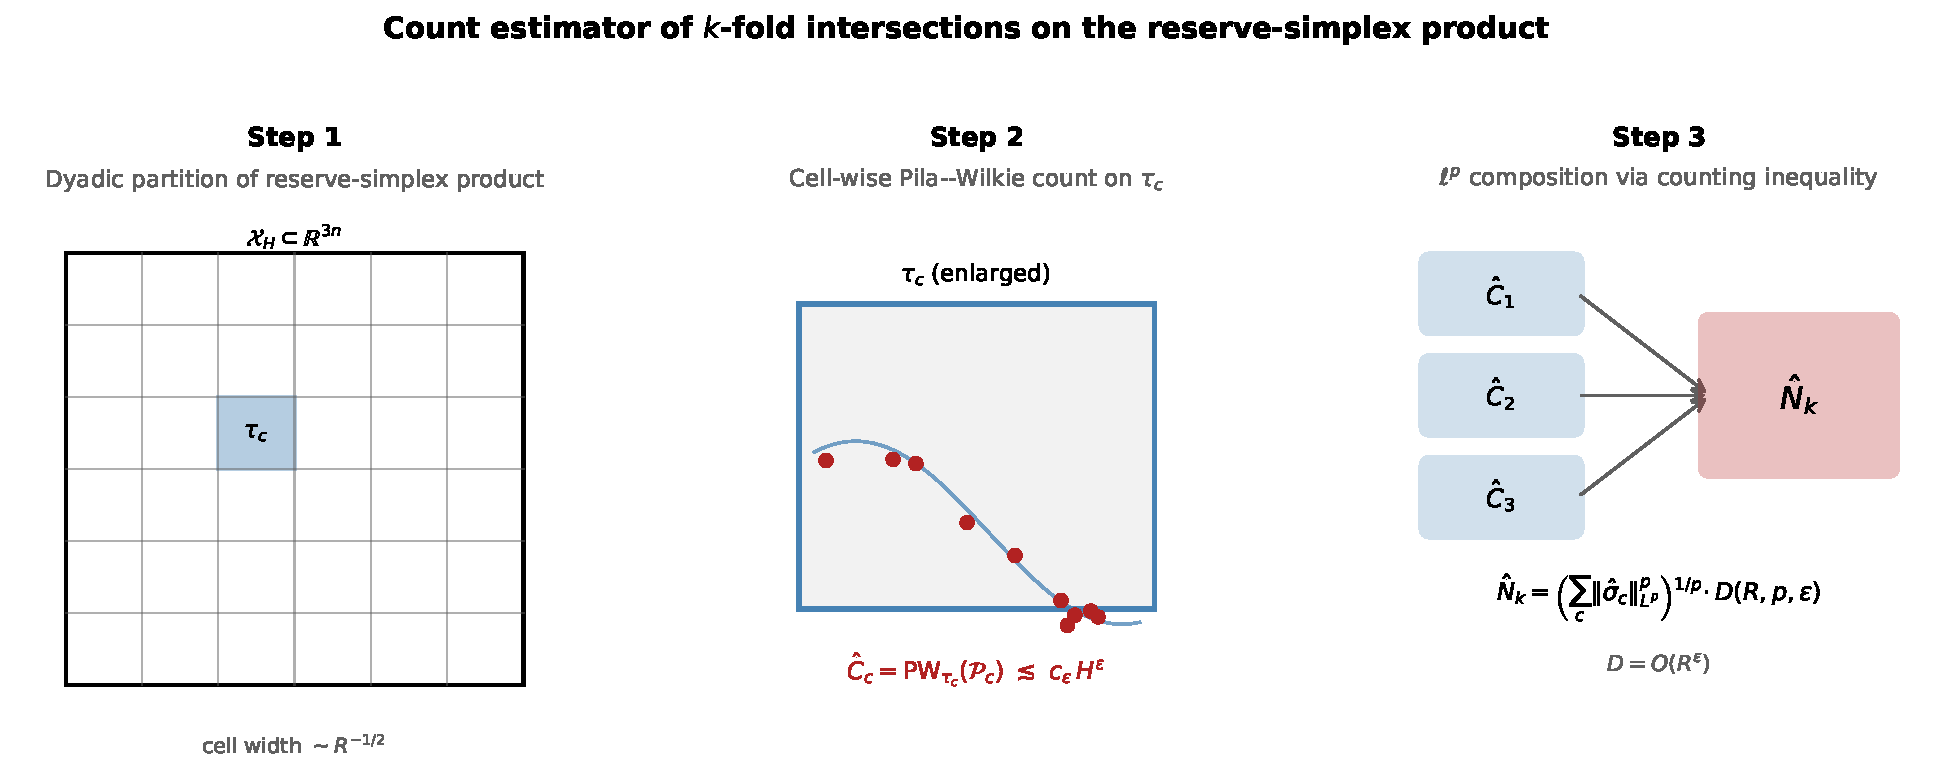
\includegraphics[width=0.95\linewidth]{figures/fig5_algorithm_flowchart.pdf}
\caption{\textbf{Count estimator of $k$-fold intersections from a
proof-of-reserves attestation set.} \emph{Step 1---dyadic
partition:} the reserve-simplex product $\mathcal{X}_H$ is split
into $O(R)$ cells $\{\tau_c\}$ of angular width $R^{-1/2}$ with
$R = 1/\delta$. \emph{Step 2---cell-wise Pila--Wilkie count:} on
each cell $\tau_c$ the sub-family
$\mathcal{P}_c = \{p_e : n_e \in \tau_c\}$ contributes a
transcendental-part count
$\hat C_c \le c_\varepsilon H^\varepsilon$ from
\citet{PilaWilkie2006}. \emph{Step 3---$\ell^p$ composition:} the
cell-wise counts compose into the final estimate
$\hat N_k = \bigl(\sum_c \|\hat\sigma_c\|_{L^p}^p\bigr)^{1/p}
\cdot D(R,p,\varepsilon)$, where $D = O(R^\varepsilon)$ carries the
intrinsic $H^\varepsilon$ loss of Theorem~\ref{thm:prior} and
Proposition~\ref{thm:lower}. The overall complexity is
$O(N_\delta \log N_\delta)$ under $N_\delta \asymp R^\alpha$ for
$\alpha \in (n{-}1, n)$: the partition dominates and the
composition step is $O(R)$ in the number of cells.}
\label{fig:alg-flowchart}
\end{figure}

A reference Python implementation in about 200 lines, together
with a worked example on the panel of Section~\ref{sec:empirics},
is included in the reproducibility archive.

\end{document}
